%======================================================================
\chapter{Algorithms and Analysis for the {\sc Closest String} Problem}\label{chapter:closest_string_problem}
%======================================================================

In the previous chapter we described MCL-WMR, a motif-recognition program that builds a weighted graph model of the input data, efficiently clusters the data to determine smaller subproblems that are likely to contain a motif, and recovers motifs by the use of a dynamic-programming algorithm.  The last step involves solving the {\sc Closest String} problem a significantly large number of times.  As described in the previous chapter, we refer to a set of strings $S$ as pairwise bounded if for all strings $a, b \in S$, $d(a,b) \leq 2d$.  Thus, the {\sc Closest String} problem reduces to discerning between pairwise bounded sets that have a center string, and if so, finding one such string $s^*$, and those sets that do not. The dynamic-programming algorithm used by MCL-WMR to solve the {\sc Closest String} problem has exponential running time and in practice is the most computational intensive step of MCL-WMR. Hence, this algorithm becomes a significant bottleneck in solving motif-recognition instances -- especially where $d$ is large relative to $\ell$. To improve upon the capability of MCL-WMR, we develop efficient heuristics to solve the {\sc Closest String} problem.  

In this chapter we study the {\sc Closest String} problem in more detail.  Smith showed several results indicating the ``alphabet size does significantly influence many pattern finding problems''  \cite[p. 51]{asmith}.   Similarly, we give strong evidence to demonstrate that the number of strings has a significant affect on the cost of solving the {\sc Closest String} problem and therefore, influences how we should attempt to solve the problem.  We investigate different methods for efficiently discerning between motif sets and decoy sets; to accomplish this task we will divide the problem into studying instances with a small number of strings, and instances with a large number of strings. 
  
Following the path of previous authors \cite{GNR01,SLC04}, we first focus on efficiently solving restricted instances of the {\sc Closest String} problem. Gramm {\em et al.}\ \cite{GNR01}  and Sze {\em et al.}\ \cite{SLC04}  gave direct, combinatorial algorithms for solving the {\sc Closest String} problem exactly for three strings.  The algorithm of the former authors considers the possible combinations of alphabet symbols that can occur for three strings, then specifies conditions for which a center string can be constructed \cite{GNR01}.  Sze {\em et al.}\ \cite{SLC04} gave a counting argument to demonstrate a condition for which a set of three strings has a center string and when it does not.  Gramm {\em et al.}\ stated that the problem of finding an efficient polynomial-time algorithm for solving the {\sc Closest String} problem on a set of four strings remains open ``due to the enormous combinatorial complexity [of the integer linear programming based solution]'' \cite[p. 13]{GNR03}.  We resolve this open problem for binary strings; specifically, we give an exact combinatorial algorithm for four binary strings.  

We also prove that {\sc Closest String} instances can be solved efficiently when the instances have a large number of strings.  Evidence for the efficiency is provided in a two-fold manner.  First, we introduce and investigate a randomized algorithm for the {\sc Closest String} problems, which we refer to as {\em CSP-Greedy}.  We prove that this randomized algorithm computes, with high probability, the {\sc Closest String} on smoothed instances up to a constant factor approximation.  Using smoothed analysis, we show the algorithm runs in $O(\ell^3)$, where $\ell$ is the string length, and achieves a $(1 + f(\epsilon, n, \ell))$ approximation guarantee, where $\epsilon > 0$ is any small value, $n$ is the number of strings, and $f(\epsilon, n, \ell) = O(\delta^n) $ for some $\delta < 1$.  

Next, we examine the $O(n\ell + nd \cdot d^d)$-time algorithm by Gramm {\em et al.}\ \cite{GNR03}, which has been shown to work very efficiently on practical instances. We explain this good performance through smoothed analysis.  Essential to our analysis is the introduction of a new perturbation model of the {\sc Closest String} model and the analysis of the Gramm {\em et al.}\ \cite{GNR03} algorithm in this model. We prove for any given {\sc Closest String} instance $I$, the average running time of this algorithm on a small perturbation of $I$ is $O(n\ell + nd \cdot d^{2 - \epsilon})$.  

We refer to the {\em cardinality} of a {\sc Closest String} instance as the number of strings in the set.  We note that the results in this chapter are complementary; the first part of this chapter will demonstrate that small, very restricted instances can be solved efficiently and the second part will show that instances that contain a large number of strings can be solved efficiently.   
 
We conclude this section by showing the applicability of this analysis to motif recognition. We extend MCL-WMR to incorporate {\em CSP-Greedy} and obtain {\em pMCL-WMR}, a program that is able to detect motifs in sets of large cardinality ({\em i.e.} instances that have 30 or more sequences) and find regulatory sequences in genomic data.  Our data shows that detecting motifs in large data sets is easier in comparison to when the number of sequences is relatively small -- a fact that gives surprising insight into this central problem in bioinformatics. 

\newpage
The main contributions in this chapter are as follows:
\begin{itemize} 
\item We give a linear-time algorithm for solving small {\sc Closest String} instances (Section \ref{sec:small_CS_insances}).
\item We describe our algorithm, {\em CSP-Greedy}, prove it achieves a 2-approximation guarantee, and give a bound on the probability that {\em CSP-Greedy} returns an optimal solution to the {\sc Closest String} instance.  Using smoothed analysis we show {\em CSP-Greedy} achieves an $1 + f(\epsilon, n, \ell)$-approximation guarantee in time $O(\ell^3)$, where $\epsilon > 0$ is any small value and $f(\epsilon, n, \ell)$ approaches zero in time that is exponential in $n$, and the expected running time of the algorithm of Gramm {\em et al.}\ \cite{GNR03} is $O(n\ell + nd \cdot d^{2 + \epsilon})$ (Section \ref{sec:large_CS_insances_v1}).
\item We show the applicability of the algorithms for solving {\sc Closest String} instances in speeding up motif detection (Section \ref{section:exp_results}).
\end{itemize}

%%%%%%%%%%%%%%%%%%%%%%%%%%%%%%%%%%%%%%%%%%%%%%%
\section{A Linear-Time Algorithm for Solving Small \\ {\sc Closest String} Instances} \label{sec:small_CS_insances}

In this section, we provide empirical evidence suggesting that the majority of decoy sets have a subset of cardinality four that is a decoy, and describe a linear-time algorithm for determining whether a set of four strings is a decoy, addressing an open problem of Gramm {\em et al.}\ \cite{GNR03}. Our empirical results together with our algorithm suggest that the majority of instances of the {\sc Closest String} problem can be solved in polynomial time.

We begin with some definitions concerning general string analysis.  Let $\ell$, $d$, and $n$ be positive integers with $d \leq \ell$. Let $\sigma_i$ be a function that returns the $i$th symbol in a string. For any symbol $\beta \in \Sigma$ let $\beta^{\ell}$ denote the length $\ell$ string of all $\beta$ symbols. Given a set of strings $S = \{ s_1, \ldots, s_n \}$, each of which has length $\ell$, the $i$th {\em column} refers to the column vector $c_i = [\sigma_i(s_1), \ldots, \sigma_i(s_n)]^T$ in the $n \times \ell$ matrix representation of $S$. 

We will be interested in the cardinality of a decoy set, that is, the number of strings contained in the set. We say set $\hat{S} \subseteq S$ is a decoy of {\em minimal cardinality} if $\hat{S}$ is a decoy set such that for all $S' \subseteq S$, if $|S'| < |\hat{S}|$, then $S'$ has a center string. 


Gramm {\em et al.}\ \cite{GNR01} refer to the process of permuting the columns of $S$ such that these are grouped by column type as {\em normalization}. A normalized instance can be derived from the input set of strings by a simple linear-time algorithm.  Given a {\sc Closest String} for the normalized set of strings, the inverse of this same permutation returns
a center string for the original input \cite{GNR01}. 

\subsection{Definitions Specific to Sets of Cardinality Four}
 
Given a binary alphabet $\Sigma = \{\alpha, \beta \}$ and a set of strings $S=\{s_1, \ldots, s_4\}$, the symbols in each column have  either two, three, or four matching symbols. Sixteen types of columns are possible in general. We say a column belongs to {\em group $i$} if it has exactly $i$ matching symbols. To reduce the number of possible types to eight, suppose without loss of generality that $s_4 = \beta^{\ell}$. Equivalently, create a new set $S'$ by performing a logical exclusive-or of each string in $S$ with $s_4$ (say $\alpha$ corresponds to boolean true). A center string for $S$ is found by performing another exclusive-or on a center string for $S'$. Let $\lambda_{abc}$ denote the number of instances of column  $(a, b, c, \beta)^T$, where $a, b, c \in \{\alpha, \beta \}$. See Table~\ref{tab:possible_columns}. Note that only columns of groups three and two need to be considered, since any center string will correspond to the majority at each column of group four.  A pair of columns are considered to be {\em identical} if a pair of strings in one column mismatch if and only if the same strings mismatch in the second column.  For example the column $[  \alpha \alpha \beta \beta ]^T$ is identical to $[\beta \beta \alpha \alpha]^T$, but neither is identical to $[\alpha \beta \beta \alpha]^T$.  

Let $\maj_i$ denote the majority of the four symbols in column $i$. That is, $\maj_i = \alpha$ if symbol $\alpha$ occurs three or more times in column $i$ and $\maj_i = \beta$ if symbol $\beta$ occurs three or more times; $\maj_i$ is undefined if $\alpha$ and $\beta$ each occur twice.  Assuming that $s_4 = \beta^{\ell}$, only the columns associated with $\lambda_{\alpha\alpha\alpha}$ are such that $\maj_i = \alpha$.

\begin{table}[t]
\begin{center}
%\begin{tabular*}{0.75\textwidth}{@{\extracolsep{\fill}}|c|c|cccc|ccc|}
\begin{tabular}{|c|c|cccc|ccc|}
\hline
Group & 
\multicolumn{1}{c|}{Four} &
\multicolumn{4}{c|}{Three} &
\multicolumn{3}{c|}{Two} \\
\hline
\# of columns. &  $\lambda_{\beta\beta\beta}$ & $\lambda_{\alpha\beta\beta}$ & $\lambda_{\beta\alpha\beta}$ & $\lambda_{\beta\beta\alpha}$ & $\lambda_{\alpha\alpha\alpha}$ & $\lambda_{\beta\alpha\alpha}$ & $\lambda_{\alpha\beta\alpha}$ &   $\lambda_{\alpha\alpha\beta}$\\
\hline
$s_1$ 		& $\beta$ & $\alpha$ & $\beta$ & $\beta$ & $\alpha$ & $\beta$ & $\alpha$ & $\alpha$ \\
$s_2$ 		& $\beta$ & $\beta$ & $\alpha$ & $\beta$ & $\alpha$ & $\alpha$ & $\beta$ & $\alpha$ \\
$s_3$ 		& $\beta$ & $\beta$ & $\beta$ & $\alpha$ & $\alpha$ & $\alpha$ & $\alpha$ & $\beta$ \\
$s_4$ 		& $\beta$ & $\beta$ & $\beta$ & $\beta$ & $\beta$ & $\beta$ & $\beta$ & $\beta$ \\
\hline
$\maj_i$ & $\beta$ & $\beta$ & $\beta$& $\beta$ & $\alpha$ & - & - & - \\
\hline
\end{tabular}
\caption[Defining the different types of columns for a set of strings with cardinality four.]{Defining the different types of columns for a set of strings with cardinality four. The values $\lambda_{\alpha\beta\beta}$ through $\lambda_{\alpha\alpha\beta}$ denote the number of columns of each type in
groups three and two.  The symbol ``-'' implies that the value is undefined at these columns.}
\end{center}
\label{tab:possible_columns}
\end{table}

%%%%%%%%%%%%%%%%%%%%%%%%%%%%%%%%%%%%%%%%%%%%%%%%%%%%%%%%%%%%%%%%%%%%%%%%%%%%%%%%%%%%%%%%%%%%%%%%%%%%%%%%%%%%%%%%%% 
\subsection{Ubiquitousness or Rarity of Bounded Decoy Sets}

We consider the relative frequency, or infrequency, of decoy sets that do not have a proper subset that is also a decoy. Our empirical results demonstrate that the relative frequency of such decoy sets is minimal, and that the majority of decoy sets contain a decoy subset of cardinality four.  Still, the results of Gramm {\em et al.}\ \cite{GNR03} imply that we cannot characterize all decoy sets of arbitrary size $n$ as having a proper subset that is a decoy. We refer to a set $Q$ of decoys, each of cardinality $n$,  as having decoys of {\em bounded cardinality} if every decoy in $Q$ has a proper subset that is a decoy.
  
\begin{proposition} \label{cb1:corollary1} Let $\Sigma$ denote an alphabet of arbitrary fixed size. If $P \neq NP$, then for any $n_0$ there exists a decoy set $S$ such that every subset of $S$ of cardinality $n_0$ has a center string. \end{proposition}

\begin{proof} Suppose otherwise. That is, there exists an $n_0$ such that
every decoy $S$ of size $n \geq n_0$
has a subset of size $n_0$ that is a decoy.
By Gramm {\em et al.}\ \cite{GNR03}, for any fixed $n_0$, 
there exists an algorithm that decides whether a set of $n_0$ strings 
is a decoy in $f(\ell,d)$ time, where $f(\ell,d)$ is polynomial in $\ell$ and $d$.
Consequently, for any set of $n \geq n_0$ strings $S$, 
we can check each of the ${{n} \choose {n_0}}$ subsets of $S$ of size $n_0$
to determine whether any is a decoy in time $O(n^{n_0} f(l,d)))$.
That is, we can determine in polynomial time whether $S$ is a decoy.
Since the {\sc Closest String} problem is NP-complete, 
this is possible only if P = NP.
\hfill $\Box$ \end{proof}

It should be noted that Proposition \ref{cb1:corollary1} does not preclude that there may exist values of $n$ such that all decoys of cardinality $n$ have a minimal decoy set of cardinality $n$.  Proposition \ref{cb1:corollary1}  implies that there does not exist a threshold $n_0$ such that every decoy set contains a minimal decoy set of cardinality at most $n_0$, if $P \not= NP$.  Although Proposition~\ref{cb1:corollary1} implies that no fixed $n_0$ exists, we conjecture that most decoys have a subset of size four that is a decoy. We provide evidence toward this property with an empirical study on random sets of binary strings which we now describe. In turn, these results motivate the need for an efficient algorithm for determining whether a set of four strings has a center string; we describe such an algorithm in Section~\ref{sec:alg}.

\begin{table}[th]
\begin{center} {\footnotesize
\begin{tabular}{|c||c|c|c||c|c|c||c|c|c|}
\hline
Number of 			& \multicolumn{3}{c||}{$\ell = 8$, $d = 3$} & \multicolumn{3}{c||}{$\ell = 10$, $d = 3$}  & \multicolumn{3}{c|}{$\ell = 15$, $d = 4$} \\
strings 	& \multicolumn{1}{c|}{$n = 6$} & \multicolumn{1}{c|}{$n = 10$} & \multicolumn{1}{c||}{$n = 12$} 
					& \multicolumn{1}{c|}{$n = 6$} & \multicolumn{1}{c|}{$n = 10$} & \multicolumn{1}{c||}{$n = 12$}  
    				& \multicolumn{1}{c|}{$n = 6$} & \multicolumn{1}{c|}{$n = 10$} & \multicolumn{1}{c||}{$n = 12$} \\
\hline
\hline
No. of valid &	443.4	&	4.6 &	88.7 &	394.4 & 9.3 & 3.6 & 101.4 & 3.5 & 2.6 \\
motif &&&&&&&&& \\
\hline
\hline
 4 		& 542.2    & 995.4  	& 991.3  	& 605.6 	& 990.7 	&  996.4 		& 898.6 	& 996.5 	&  997.4  	\\
 5  		& 12.4     	& 0 			& 0   	 	& 7  			&  0  		&  0 				& 4.1  		&  0  		&  0 	\\
 6 		& 2     		& 0   		& 0 			& 0.2  		&  0 			&  0  			& 0.8  		&  0 			&  0  \\
 7    		& -     		& 0   		& 0  			& -  			&  0 			&  0 				& -  			&  0 			&  0 	\\
 8  		& -     		& 0   		& 0  			& -  			&  0 			&  0 				& -  			&  0 			&  0	\\	
 9   		& -     		& 0   		& 0  			& -  			&  0 			&  0 				& -  			&  0 			&  0	\\	
 10    	& -     		& 0  			& 0   		& -  			&  0 			&  0 				& -  			&  0  		&  0	\\
 11    	& -     		& -  			& 0   		& -  			&  -			&  0 				& -  			&  - 			&  0	\\
 12       & -     		& -  			& 0  			& -  			&  -			&  0    			& -  			&  - 			&  0	\\
\hline
\end{tabular} }
\end{center}
\caption[Experimental data illustrating the ubiquitousness of decoy sets of cardinality four.]{Experimental data illustrating the ubiquitousness of decoy sets of cardinality four. Data obtained from calculating the average of 10 experiments that obtain a random sample, without replacement, of 1000 sets of strings and determining the size of the minimal decoy contained in each set decoy obtained in the sample.  The first column is the cardinality of the minimum decoy set. }
\label{decoy_table}
\end{table} 

We empirically investigate the rarity of the occurrence of decoy sets of cardinality $n$ for which the cardinality of a minimal decoy set is large relative to $n$. We sampled without replacement 1000 times from the set of all possible pairwise-bounded sets of binary, length-$\ell$ strings; each set sampled has exactly $n$ strings taken from the binary alphabet.  We varied the values for $n$, $\ell$ and $d$.  For each sample set, we determined whether the set is a decoy or a valid motif, with respect to the value of $d$, and determined the cardinality of the minimum decoy set.  We repeated this experiment ten times and calculated the mean values obtained. Table \ref{decoy_table} outlines this data. One significant empirical trend demonstrates that as the number of strings increased, the number of decoys that do not contain a minimal decoy of cardinality four became exponentially smaller; when $n$ was ten and twelve the number of minimal decoys of size larger than four was zero.  The only value of $n$ for which decoys of size $n$ were seen was six.  Further, the total number of decoys in 900,000 sets of strings sampled was approximately 1,500.  In summary, the empirical results suggest that a large percentage of binary decoys can be characterized by containing a minimal decoy set of size four, the smallest size possible, further motivating the main results in the following subsection.  

\subsection{Finding a Center String for a Set of Four Strings} \label{sec:alg}
 
The only previous polynomial-time solution for finding a center string of a set of four strings was intended more to demonstrate the fixed-parameterized tractability of the problem rather than to provide an efficient solution \cite{GNR03}. As acknowledged by its authors, the corresponding description (for which many details are omitted) results in an algorithm with extremely high  (although theoretically linear) run time and, furthermore, does not lend itself well to simple or practical implementation. We present a simple linear-time algorithm for finding a center string of a set of four binary strings or determining that the set is a decoy. After describing the algorithm, we prove its correctness and  show its worst-case run time is $O(\ell)$ for any arbitrary $d$.

Given a set of binary strings $S = \{s_1, \ldots, s_4\}$,  algorithm {\sc BinaryClosestString4}  identifies a center string $s^*$ for $S$ if one exists. Again, to simplify the algorithm's description, suppose $s_4 = \beta^{\ell}$. The algorithm greedily assigns symbols to $s^*$, one symbol at a time. Each column $c_i$ is initially considered to be {\em free};
that is, no symbol has been assigned to $\sigma_i(s^*)$. Once it is assigned a symbol, we say column $c_i$ is {\em fixed} and its value is not modified again.
%The first four values in a column may have either two, three, or four matching 
%symbols.
%We say a column belongs to group $i$ if it has exactly $i$ matching symbols. 
%Eight types of columns are possible. 
%Let $\lambda_{\beta\beta\beta}$ through $\lambda_{\alpha\alpha\beta}$ 
%denote the respective number of columns of each type.
%See Table~\ref{tab:phase3}.
The algorithm has three phases in which columns of groups four, three, 
and two are fixed, respectively.

{\bf Phase One.}
Fix symbols of $s^*$ in all columns of group four such that these agree with 
the symbol of the corresponding column.

{\bf Phase Two.}
The symbols of $s^*$ in columns of group three are fixed sequentially. 
Say the first $i-1$ columns of group three have been fixed and consider the $i$th such column.
Let $s_j$ denote the string in $S$ that disagrees with the
remaining three strings in this column.
Let $s^+$ denote the string 
given by the symbols of $s^*$ in the fixed columns 
and the symbols of $s_j$ in the free columns.
If $s^+$ is a center string for $S$, then let $s^* = s^+$ and return $s^*$.
Otherwise, fix the current column of $s^*$ to agree with the majority
and continue to the next column of group three.

{\bf Phase Three.}
If phase three is reached, then only columns of group two remain,
of which at most three types may be present.
The free columns are fixed by selecting the number of columns
of each type that will be assigned symbol $\alpha$ versus $\beta$.
That is, a solution for columns of group two corresponds to a triple of integers
$(x,y,z)$,
where $x \in [0,\lambda_{\beta\alpha\alpha}]$
denotes the number of columns of type $\lambda_{\beta\alpha\alpha}$
that will be assigned the symbol $\alpha$ 
and $\lambda_{\beta\alpha\alpha}-x$ represents the number that will 
be assigned the symbol $\beta$.
The variables $y$ and $z$ are defined analogously.
See Table~\ref{tab:phase3}.
We denote the corresponding string by $s^*_{x,y,z}$.
Therefore, the problem reduces to identifying an integer triple $(x,y,z)$
selected from the region $R = [0, \lambda_{\beta\alpha\alpha}]
\times [0, \lambda_{\alpha\beta\alpha}] 
\times [0, \lambda_{\alpha\alpha\beta}]$
that minimizes
\begin{equation}
\label{eqn:minimizeObj}
f(x,y,z) = \max_{s_i \in S} d(s_i, s^*_{x,y,z}) ,
\end{equation}
where
\begin{subequations}
\begin{align}
d(s_1, s^*) & = \lambda_{\alpha\beta\beta} + x + \lambda_{\alpha\beta\alpha} - y
+ \lambda_{\alpha\alpha\beta} - z , 
\label{eqn:phase3Constraint1}
\\
d(s_2, s^*) & = \lambda_{\beta\alpha\beta} + \lambda_{\beta\alpha\alpha} - x 
+ y + \lambda_{\alpha\alpha\beta} - z , 
\label{eqn:phase3Constraint2}
\\
d(s_3, s^*) & = \lambda_{\beta\beta\alpha} + \lambda_{\beta\alpha\alpha} - x 
+ \lambda_{\alpha\beta\alpha} - y + z , 
\label{eqn:phase3Constraint3}
\\
d(s_4, s^*) & = \lambda_{\alpha\alpha\alpha} + x + y + z .
\label{eqn:phase3Constraint4}
\end{align}
\end{subequations}
The string $s^*_{x,y,z}$ does not actually need to be constructed since
the corresponding value of \eqref{eqn:minimizeObj} is obtained in constant time
upon fixing values for $x$, $y$, and $z$.

\begin{table}
\centering
%\begin{tabular*}{0.75\textwidth}{@{\extracolsep{\fill}}|cc|c|cccc|ccc|}
\begin{tabular}{|cc|c|cccc|ccc|}
\hline
\multicolumn{2}{|r|}{Column Group} &
\multicolumn{1}{c|}{Four} &
\multicolumn{4}{c|}{Three} &
\multicolumn{3}{c|}{Two} \\
\multicolumn{2}{|r|}{Algorithm Phase} &
\multicolumn{1}{c|}{1} &
\multicolumn{4}{c|}{2} &
\multicolumn{3}{c|}{3} \\
\hline
\multicolumn{2}{|r|}{Number of Columns} &
$\lambda_{\beta\beta\beta}$ &
$\lambda_{\alpha\beta\beta}$ &
$\lambda_{\beta\alpha\beta}$ &
$\lambda_{\beta\beta\alpha}$ &
$\lambda_{\alpha\alpha\alpha}$ &
$\lambda_{\beta\alpha\alpha}$ &
$\lambda_{\alpha\beta\alpha}$ &
$\lambda_{\alpha\alpha\beta}$ \\
%used to be & & & a & b & c & d & e & f & g \\
\hline
\multirow{4}{*}{Set $S$} 
& $s_1$ & $\beta$ & $\alpha$ & $\beta$ & $\beta$ &
$\alpha$ & $\beta$ & $\alpha$ & $\alpha$ \\
& $s_2$ & $\beta$ & $\beta$ & $\alpha$ & $\beta$ &
$\alpha$ & $\alpha$ & $\beta$ & $\alpha$ \\
& $s_3$ & $\beta$ & $\beta$ & $\beta$ & $\alpha$ &
$\alpha$ & $\alpha$ & $\alpha$ & $\beta$ \\
& $s_4$ & $\beta$ & $\beta$ & $\beta$ & $\beta$ & 
$\beta$ & $\beta$ & $\beta$ & $\beta$ \\
\hline
Center string & $s^*$ & $\beta$ & $\beta$ & $\beta$ & $\beta$ & $\alpha$ &
$x$ & $y$ & $z$ \\
\hline
\end{tabular}
\caption[Illustration of the center string found by algorithm {\sc BinaryClosestString4}]{The center string found by algorithm {\sc BinaryClosestString4} 
(if one exists) is displayed in the last row. The center string is denoted as $s^*$.
The values $\lambda_{\beta\beta\beta}$ 
through $\lambda_{\alpha\alpha\beta}$ 
denote the number of columns of each type 
and functions $x$, $y$, and $z$ denote the number of occurrences of symbol
$\alpha$ in the corresponding column as derived by the algorithm.}
\label{tab:phase3}
\end{table}

Instead of evaluating all integer combinations for $(x,y,z)$
(requiring $O(\ell^3)$ time),
we identify a set $T \subseteq \mathbb{Q}^3 \cap R$ 
containing a constant number of triples
such that the optimal (possibly non-integer)
solution to \eqref{eqn:minimizeObj} is a triple in $T$.
Interpreted geometrically, 
\eqref{eqn:phase3Constraint1} through \eqref{eqn:phase3Constraint4}
correspond to four respective hyperplanes in $\mathbb{R}^4$
whose maximum, $f(x,y,z)$, defines a surface.
Let
\begin{align}
x_0 & = \frac{1}{4} \left(
- \lambda_{\alpha\beta\beta} + \lambda_{\beta\alpha\beta}
+ \lambda_{\beta\beta\alpha} - \lambda_{\alpha\alpha\alpha}
+ 2\lambda_{\beta\alpha\alpha} \right) ,
\nonumber \\
y_0 & = \frac{1}{4} \left(
  \lambda_{\alpha\beta\beta} - \lambda_{\beta\alpha\beta}
+ \lambda_{\beta\beta\alpha} - \lambda_{\alpha\alpha\alpha}
+ 2\lambda_{\alpha\beta\alpha} \right) ,
\nonumber \\
z_0 & = \frac{1}{4} \left(
  \lambda_{\alpha\beta\beta} + \lambda_{\beta\alpha\beta}
- \lambda_{\beta\beta\alpha} - \lambda_{\alpha\alpha\alpha}
+ 2\lambda_{\alpha\alpha\beta} \right) .
\label{eqn:phase3Sol}
\end{align}
If $(x_0,y_0,z_0) \in R$, then let $T = \{(x_0, y_0, z_0)\}$.
Otherwise, let $T$ denote the set of triples that correspond to
$x$-, $y$-, and $z$-coordinates of vertices of the
intersection of the surface defined by 
\eqref{eqn:minimizeObj} with the boundary of $R$.
If this intersection is empty, then it follows that no center string exists.

For each triple $(x,y,z) \in T$, 
evaluate the integer triples within unit $L_\infty$ distance 
of $(x,y,z)$ in region $R$. 
That is, for every $(x,y,z) \in T$, consider the integer triples in 
$[ \max(0, x-1), \min(x+1, \lambda_{\beta\alpha\alpha}) ]
\times [ \max(0, y-1), \min(y+1, \lambda_{\alpha\beta\alpha}) ]
\times [ \max(0, z-1), \min(z+1, \lambda_{\alpha\alpha\beta}) ]$,
of which there are at most eight.
Compute \eqref{eqn:minimizeObj}
for each such integer triple $(x,y,z)$
and store the corresponding minimizing string $s^*_{x,y,z}$.
Let $s^* = s^*_{x,y,z}$.

%If $x_0$ (respetively, $y_0$ or $z_0$) 
%lies outside the range of feasible solutions 
%$[0, \lambda_{\beta\alpha\alpha})]$, then $x_0$
%is assigned a new value corresponding to the nearest endpoint of that interval.
%For example, if $x_0 < 0$ then set $x_0 = 0$.
%As a result, the values of $y_0$ and $z_0$ are updated by one of four
%possible values, from which the optimum is selected.
%These four new potential points are found by solving
%for $t$ in each of the four sets of equations, depending on which of 
%$x_0$, $y_0$, or $z_0$ has a new fixed value.
%\begin{subequations}
%\begin{align}
%x_1(t) = t+\frac{1}{2}(-a+c+e-f)
%& y_1(t) = t+\frac{1}{2}(-b+c+e-g)
%& z_1(t) = t ,
%\\
%x_2(t) = -t+\frac{1}{2}(b-d+e+g)
%& y_2(t) = -t+\frac{1}{2}(a-d+f+g)
%& z_2(t) = t ,
%\\
%x_3(t) = t+\frac{1}{2}(-a+c+e-g)
%& y_3(t) = t+\frac{1}{2}(-a+c+e-g)
%& z_3(t) = t ,
%\\
%x_4(t) = -t+\frac{1}{2}(b-d+e+g)
%& y_4(t) = t+\frac{1}{2}(-b+c+f-g)
%& z_4(t) = t .
%\end{align}
%\end{subequations}
%
%The remaining optimization corresponds to a set of four planes in 
%$\mathbb{R}^3$. Again, the optimal solution lies at one of two vertices
%on the 1-level (maximum) surface.
%If the lower of these points lies outside $R$,
%the corresponding variable, say $y$ is truncated, and the search
%continues on a set of four lines in $\mathbb{R}$, for which the optimal
%solution lies at one of three vertices on the 1-level.
%Again, the optimal remaining varibles 
%then the best solution inside $R$

{\bf Termination.}
Consider the maximum distance between $s^*$ and a string in $S$,
{\em i.e.}, the minimum (integer) value of \eqref{eqn:minimizeObj}.
If this value is at most $d$, 
then $s^*$ is returned as a center string for $S$. 
Otherwise, $S$ is a decoy set and no center string exists.

We now demonstrate that algorithm {\sc BinaryConsensus4} correctly returns a 
center string $s^*$ for every set $S$ that is a valid motif set.
Furthermore, this is achieved in $O(\ell)$ time, independent of $d$.
The proof of Theorem~\ref{thm:algCorrectness} refers to 
Lemmas~\ref{lem:phase2} and~\ref{lem:phase3} which follow.

\begin{theorem}
\label{thm:algCorrectness}
Given any $d \in \mathbb{Z}^+$, any $\ell \in \mathbb{Z}^+$,
and any set $S$ of four binary strings of length $\ell$,
algorithm {\sc BinaryConsensus4} 
returns a center string for $S$ with degeneracy parameter $d$
if one exists or returns that $S$ is a decoy
in $O(\ell)$ time.
\end{theorem}

\begin{proof}
The correctness of Phase One is straightforward.
The correctness of Phase Two follows by induction on $i$ 
using Lemma~\ref{lem:phase2}.
Consequently, if $S$ has a center string, then either one has been found 
by the end of Phase Two (i.e., $s^* = s^+$), 
or there exists a center string $s^*$ such that
$\sigma_x(s^*) = \maj_x$ for all columns of groups three and four.
The optimal solution for the remaining free columns is found in Phase Three.
The correctness of Phase Three follows by Lemma~\ref{lem:phase3}.
Therefore, algorithm {\sc BinaryClosestString4} returns a center string $s^*$
if one exists, and returns that no center string exists otherwise.

Each phase requires a single pass through the columns of $S$.
Phase One simply requires counting the number of columns of each type.
Phase Two also requires maintaining the twelve distances $d(s_i, s^+_j)$
for each $\{i, j\} \subseteq \{1, \ldots, 4\}$, 
where $s^+_j$ denotes $s^+$ for which the free columns are
defined according to $s_j$ 
(as described in Phase Two of algorithm {\sc BinaryConsensus4}).
Every time a column of group three is fixed,
each of these twelve values can be updated in constant time.
Phase Three simply requires counting the number of columns of each type.
Since \eqref{eqn:minimizeObj} 
is defined by the maximum of four hyperplanes and
region $R$ is bounded by three pairs of parallel planes,
the number of triples in $T$ is constant and, furthermore, the coordinates
of these triples are straightforward to compute in constant time.
Finally, since any point in $\mathbb{R}^3$ has at most eight integer points 
within unit $L_\infty$ distance from it, the set of integer triples evaluated
is also computed in constant time and space.
Therefore, algorithm {\sc BinaryConsensus4} terminates in $O(\ell)$ time.
\hfill $\Box$ \end{proof}

\begin{definition}[Majority-Rule Property]
We say property $P(i)$ holds for a set $S$ of four binary strings 
if and only if either
\begin{enumerate}
\item $S$ is a decoy, or
\item there exists a center string for $S$ for which
the first $i$ columns of group three have value $\maj_i$.
\end{enumerate}
\end{definition}

\begin{lemma}
\label{lem:phase2}
Let $S = \{s_1, \ldots, s_4\}$ denote a set of four binary strings
that has $m$ columns of group three.
If $P(i)$ holds for some $i \in \{0, \ldots , m-1\}$ 
and $s_j \in S$ denotes the string that mismatches in the $(i+1)$st 
column of group three, then either
\begin{enumerate}
\item $P(i+1)$ holds for $S$, or
\item $s^+$ is a center string for $S$,
\end{enumerate}
where $\sigma_x(s^+) = \maj_x$ in the first $i$ columns of group three
and $\sigma_x(s^+) = \sigma_x(s_j)$ in the remaining columns.
\end{lemma}

\begin{proof}
If $s^+$ is a center string for $S$ then the claim holds.
Similarly, if $S$ is a decoy then $P(i+1)$ is true and the claim holds.
Therefore, suppose $S$ is not a decoy and $s^+$ is not a center string for $S$.
By $P(i)$, $S$ has a center string $s^*$ 
for which the first $i$ columns of group three have value $\maj_x$.
Let $k$ denote the index of the $(i+1)$st column of group three.

{\it Case 1.} 
Suppose $\sigma_k(s^*) = \maj_k$.
Therefore, $P(i+1)$ is true, and the claim holds.

{\it Case 2.} 
Suppose $\sigma_k(s^*) \neq \maj_k$. That is, $\sigma_k(s^*) = \sigma_k(s_j)$.
Since $s^+$ is not a center string, 
$s^*$ and $s^+$ must differ in at least one column; 
let $k'$ denote the index of such a column.
Let $s^{**}$ denote a string of length $\ell$ 
such that $\sigma_x(s^{**}) \neq \sigma_x(s^*)$ for $x \in \{k, k'\}$
and $\sigma_x(s^{**}) = \sigma_x(s^*)$ otherwise.
That is, 
$\sigma_k(s^{**}) = \maj_k$.
Thus, $d(s_j, s^{**}) = d(s_j, s^*)$ and, furthermore,
$$\forall x \in \{1, \ldots, 4\}, \ d(s_x, s^{**}) \leq d(s_x, s^*) .$$
Therefore, $s^{**}$ is a center string for $S$,
$P(i+1)$ is true, and the claim holds. \hfill $\Box$ \end{proof} 

\begin{lemma}
\label{lem:phase3}
%Let $s^*$ denote a sequence of length $l$ for which 
%all columns of groups three and four are fixed with $\sigma_x(s^*) = \maj_x$ 
%and all columns of group two are free.
There exists an integer triple $(x,y,z) \in [0,\lambda_{\beta\alpha\alpha}] 
\times [0,\lambda_{\alpha\beta\alpha}] \times [0,\lambda_{\alpha\alpha\beta}]$
%corresponding to an assignment of symbols 
%to the free columns of $s^*$ 
that minimizes \eqref{eqn:minimizeObj}
and is within unit $L_\infty$ distance from a triple in $T$,
where set $T$ contains either \eqref{eqn:phase3Sol}
or the set of triples that correspond to vertices of the
intersection of the surface defined by 
\eqref{eqn:minimizeObj} with the boundary of $R$.
\end{lemma}

\begin{proof}
Since no two of the hyperplanes 
induced by \eqref{eqn:phase3Constraint1} through \eqref{eqn:phase3Constraint4}
are parallel,
$f(x,y,z)$ is a convex function whose surface includes 
a unique simplicial vertex 
located at the point of intersection of these four hyperplanes.
Furthermore, this point minimizes $f(x,y,z)$ 
since $f$ is increasing as it tends to infinity in any direction.
Thus, $f(x,y,z)$ is minimized at a unique (possibly non-integer) point
found by solving for $x$, $y$, and $z$ in
\begin{equation}
\label{eqn:phase3Eq}
d(s_1, s^*) = d(s_2, s^*) = d(s_3, s^*) = d(s_4, s^*) . 
\end{equation}
The constraints of \eqref{eqn:phase3Eq} corresponds to a system of three linear
equations with the unique solution \eqref{eqn:phase3Sol}.

Since the coefficients of $x$
in \eqref{eqn:phase3Constraint1} through \eqref{eqn:phase3Constraint4}
are all $\pm 1$, function $f(x,y,z)$ has slope $\pm 1$ along the $x$-axis
for any fixed $y$ and $z$.
The same holds for any fixed $x$ and $y$ or any fixed $x$ and $z$.
Consequently, since $f(x,y,z)$ is convex, a minimum integer solution to 
\eqref{eqn:minimizeObj} lies within unit $L_\infty$ distance 
of its non-integer solution.
The set $T$ contains either the unique minimum \eqref{eqn:phase3Sol}
(if it lies within region $R$) 
or the set of triples that correspond to vertices of the
intersection of the surface defined by 
$f(x,y,z)$ with the boundary of $R$, 
one of which must minimize $f(x,y,z)$ over $R$.
Therefore, the claim holds. \hfill $\Box$ \end{proof}

We have obtained a linear-time algorithm for solving the {\sc Closest String} decision problem for four binary strings, and considered the relative frequency of decoy sets that do not have a proper subset that is also a decoy.  Our results generalize previous work and answer some open problems proposed in \cite{GNR01}.  Further, our empirical results demonstrate that the majority of decoy sets contain a decoy subset of cardinality four, suggesting that majority of decoy sets can be characterized as having a decoy set of cardinality four.  Such a characterization would allow the {\sc Closest String} problem to be solved efficiently with high probability.

%%%%%%%%%%%%%%%%%%%%%%%%%%%%%%%%%%%%%%%%%%%%%%%%%%%%%%%%%%%%%%%%%%%%%%%%%%%%%%%%%%%%%%%%%%%%%%%%%%%%%%%%%%%%%%%%%% 
%%%%%%%%%%%%%%%%%%%%%%%%%%%%%%%%%%%%%%%%%%%%%%%%%%%%%%%%%%%%%%%%%%%%%%%%%%%%%%%%%%%%%%%%%%%%%%%%%%%%%%%%%%%%%%%%%% 

\section{Smoothed Analysis of {\sc Closest String} Instances} \label{sec:large_CS_insances_v1}

Up to this point in this chapter, we have restricted interest to {\sc Closest String} instances where the cardinality of the instances are small.  Now we consider the opposing problem: solving instances that have a large number of strings. Using smoothed analysis, we demonstrate that {\sc Closest String} instances can be efficiently solved in practice. To the best of our knowledge, this is the first analysis of a natural random model of the {\sc Closest String} problem. In this section, we give two smoothed analysis results.  

Several other papers discuss the smoothed complexity of continuous problems \cite{BD02,DST02}  and of discrete problems \cite{DDM03,Ma08}.  The smoothed complexity of other string and sequence problems has been considered by Andoni and Krauthgamer \cite{AK}, Manthey and Reischuk \cite{MR05}, and Ma \cite{Ma08}.  Andoni and Krauthgamer \cite{AK} study the smoothed complexity of sequence alignment by the use of a novel model of edit distance; their results demonstrate the efficiency of several tools used for sequence alignment, most notably PatternHunter \cite{MTL}. Manthey and Reischuk gave several results considering the smoothed analysis of binary search trees \cite{MR05}.  Ma demonstrated that a simple greedy algorithm runs efficiently in practice for {\sc Shortest Common Superstring} \cite{Ma08}. 

We use smoothed analysis to prove that the {\sc Closest String} problem can be efficiently and accurately solved in practice by two different algorirthms, when the number of strings is significantly large.  We present two perturbation models, and analyze the expected approximation for {\em CSP-Greedy} and the expected running time for a well-known, fixed parameter tractability algorithm.  

First, we describe our algorithm, {\em CSP-Greedy}, prove it achieves a 2-approximation guarantee, and give a bound on the probability that {\em CSP-Greedy} returns an optimal solution to the {\sc Closest String} instance.  We show that {\em CSP-Greedy} achieves an $1 + f(\epsilon, n, \ell)$-approximation guarantee in time $O(\ell^3)$, where $\epsilon > 0$ is any small value and $f(\epsilon, n, \ell)$ approaches zero in time that is exponential in $n$.  

Next, we explain the good performance of the $O(n\ell + nd \cdot d^d)$-time algorithm by Gramm {\em et al.}\ \cite{GNR03} through smoothed analysis.  The algorithm is based on an efficient breadth-first search of all possible solutions; their original analysis showed the size of the breadth-first search is bounded by $(d + 1)^d$, however, the empirical analysis suggested that the expected size of the search tree is on the order of $3d$.  We give an analytical explanation of these results.  Imperative to our analysis is the introduction of a perturbation model of the {\sc Closest String} model and the probabilistic analysis of the $O(n\ell + nd \cdot d^d)$ time algorithm by Gramm {\em et al.}\ \cite{GNR03}. We show for any given {\sc Closest String} instance $I$, the average running time of this algorithm on a small perturbation of $I$ is $O(n\ell + nd \cdot d^{2 - \epsilon})$. 

\subsection{A Randomized Algorithm for {\sc Closest String}}

Our randomized algorithm, which we refer to as {\em CSP-greedy}, begins with a majority string $s$, then successively updates $s$ to make it closer to at least one string in $S$ that does not have $s$ as a center string.  We do a maximum number of $\ell$ cumulative updates to $s$. After this point, if a center string is not determined, then the process is repeated.  If a set of strings $S$ does not have a center string with respect to some value of $d$, then ``not found'' will always be returned but if it is a motif set, then with some probability a center string is returned. This probability depends on the number of times we repeat the search.  We prove that {\em CSP-Greedy} achieves a 2-approximation guarantee, and give a bound on the probability that {\em CSP-Greedy} returns an optimal solution to the {\sc Closest String} instance.

In \cite{Sch99}, Sch\"{o}ning considers the following simple probabilistic algorithm for solving the NP-complete problem of $k$-SAT: randomly choose a starting assignment and subsequently augment this initial assignment until a satisfying one is obtained.  Papadimitriou introduced this random paradigm in the context of 2-SAT and obtained an expected quadratic time bound \cite{pap91}.  These type of algorithms are referred to as Monte Carlo algorithms with one-sided error; a useful property of such algorithm is that the error probability can be made arbitrarily small with repeated independent random repetitions of the search process. We analyze a similar probabilistic approach for the {\sc Closest String} problem.  

{\em CSP-Greedy} begins with a string $s_{maj, 0}$ randomly selected from all majority strings and iteratively augments the string so that it is closer to one of the strings in $S$.  We let $s_{maj, i}$ be $s_{maj, 0}$ after it has been updated $i$ times.  At iteration $i + 1$, we obtain the string $s_{maj, i + 1}$ by augmenting $s_{maj, i}$ so that it has smaller Hamming distance to at least one string $s_k$ in $S$ where $d(s_k, s_{maj, i}) > \Delta d$. This process is repeated $\ell$ times at which point the process is restarted if there is at least one string $s_k$ in $S$ where $d(s_k, s_{maj, \ell}) > \Delta d$.  

Let $t$ be the number of times a random majority string is chosen and augmented $\ell$ times. Later in the section we define $t$ in terms of the parameters $\ell$, $n$, and $d$.   In order to determine a center string corresponding to the optimal closest distance, this search process is repeated from $\Delta d = 0$ to $\ell$.

\begin{algorithm*}[h]
\caption{Procedure {\em augment}}
\begin{algorithmic}
\STATE {\bf Input: } A set $S$ of $n$ $\ell$-length strings, parameter $d$.
\STATE {\bf Output:} A $\ell$-length string $s$ or ``not found'' 
\STATE Let $\mathcal{S}$ be the set of all $\ell$-length majority strings
\STATE Select $s_{maj, 0}$ randomly from $\mathcal{S}$.
\STATE {\bf For} $i = 0, \ldots, \ell$:
\STATE \hspace{5mm} {\bf If} $d(s_{maj, i}, s_j) \leq d$ for all $s_j \in S$ then return $s$ and terminate. 
\STATE \hspace{5mm} {\bf Else} $P = \{j: s_j \in S \mbox{ and } d(s_j, s_{maj, i}) > d \}$ 
\STATE \hspace{5mm} Choose a $p$ at random from $P$, and $1 \leq k \leq \ell$ such that $s_p(k) \ne s_{maj, i}(k)$
\STATE \hspace{5mm} Set $s_{maj, i + 1}$ to be equal to $s_p$ at position $k$ and equal to $s_{maj, i}$ at all other 
\STATE \hspace{5mm} positions 
\STATE Return ``not found''
\end{algorithmic}
\end{algorithm*}

\begin{algorithm}[h]
\caption{CSP-Greedy Algorithm}
\begin{algorithmic}
\STATE {\bf Input: } A set $S$ of $n$ $\ell$-length binary strings.
\STATE {\bf Output:} A $\ell$-length string $s$ 
\STATE {\bf For} $\Delta d$ each from 0 $\rightarrow$ $\ell$ 
\STATE \hspace{5mm} {\bf Repeat} {\em augment} $t$ times with parameter $\Delta d$
\end{algorithmic}
\end{algorithm}

We give worst-case bounds on the approximation guarantee of {\em CSP-Greedy}.  Also, we present examples of inputs for which the algorithm performs poorly and hence, give lower bounds on the approximation guarantee.  

\begin{proposition} \label{2approx_theorem} The approximation ratio of the CSP-Greedy algorithm is at most 2 for any alphabet size $|\Sigma|$. \end{proposition}

\begin{proof} Since {\em CSP-Greedy} begins with a randomly selected majority string, it is sufficient to show that for any set of strings $S$ the maximum distance from any majority string to any string in $S$ is twice the optimal closest distance.  Let $S$ be a set of strings with optimal closest distance equal to $d_{opt}$.  Without loss of generality assume $0^{\ell}$ is a closest string for $S$ and hence the maximum number of non-zero positions in each string $s_i \in S$ is at most $d_{opt}$.  By the pigeonhole principle, the maximum number of positions containing greater than $n/2$ non-zero positions in a given column is at most $2d_{opt}$. Therefore, any majority string can have at most $2d_{opt}$ non-zero positions and is at distance at most $2d_{opt}$ from each string in $S$.  \hfill $\Box$  \end{proof}

\noindent The following example shows the 2-approximation guarantee is tight: $S = \{10000001111,$ $01000001111, 11111111111, 11111111111\}$, where the majority string is $c^*_1 = 11111111111$ and the optimal closest distance is $\ell/4$. On the first iteration the majority string could be altered to $c^*_2 = 01111111111$.  On the second iteration we could choose to alter this sequence back to $c^*_1$. It is possible to alternate between $c^*_1$ and $c^*_2$ and end up returning $c_1^*$, with closest distance $\ell/2$ or twice the optimal.

\subsubsection{Probabilistic Analysis of {\em CSP-Greedy}}
 
The process of augmenting a randomly selected majority string $\ell$ times or until a closest string is found can be viewed as a Markov chain.  This abstraction will be useful in achieving an upper bound on the probability that {\em CSP-Greedy} returns an optimal solution. 

Let a set $S$ be {\em uniquely satisfiable} if there exists exactly one string $s^*$ where $d(s_i, s^*) \leq d$ for all $s_i \in S$. If $S$ is an instance that does not have a string $s$ such that $d(s, s_i) \leq d^*$ for all $s_i \in S$, then procedure {\em augment} will return ``not found''.  So we assume otherwise, that the set $S$ is uniquely satisfiable and denote the probability of obtaining $s^*$ when $\Delta d = d^*$ as $p_s$. If $s_{maj, i}$ is not equal to $s^*$ then there is at least one letter of $s_{maj, i}$ that can be changed so that $d(s_{maj, i}, s^*)$ decreases by one; the probability of this occurring is at least $1/\ell$.  Denote $X_i \in \{0, 1, \ldots, \ell\}$ ($i = 0, 1, \ldots$) as the random variable that is equal to the Hamming distance between $s_{maj, i}$ and $s^*$, where $i$ is the number of iterations of the {\em augment} procedure.  Each time a position is selected and the value of that position is augmented, either the Hamming distance is increased or decreased by one.

The process $X_0, X_1, X_2, \ldots$ is a Markov chain with a barrier at state $\ell$ and contains varying time and state dependent transfer probabilities. This process is overly complicated and we instead choose to analyze the following process: $Y_0, Y_1, Y_2, \ldots$,  where $Y_i$ is the random variable which is equal to the state number after $i$ steps and there exist infinitely many states.  Initially, this Markov chain is started like the stochastic process above ({\em i.e.}\ $Y_0 = X_0$).  As long as the inner loop is iterating, we let $Y_{i+1} = X_i - 1$  if the process decreases the Hamming distance between $s_{maj, i}$ and $s^*$ by one; and $Y_{i+1} = X_i + 1$ otherwise.  After the loop exits, we continue with the same transfer probabilities. By induction on $i$, it is clear that for each $i$, $X_i \leq Y_i$, and it follows that $p_s$ is at least $\Pr[\exists t \leq \ell : Y_t = 0]$.    

We made the assumption that the set was uniquely satisfiable, however, this assumption is not needed -- the random walk may find another center string while not in the terminating state but this possibility only increases the probability the algorithm terminates.

The following asymptotic estimation is used in the proof of the next theorem. 

\begin{fact} \label{fact1} For $i > 0$ and $j > 0$ the following asymptotic estimation holds: \begin{eqnarray}\label{eqn1}\sum_{i = 0}^{j} {{2i + j}\choose{i}} \left( \frac{\ell - 1}{\ell}\right)^{i} \left( \frac{1}{\ell}\right)^{i + j} \asymp \left( \frac{1}{ \ell - 1}\right)^j.\end{eqnarray} \end{fact}

\begin{proof} We set $i = \phi j$ and estimate the summand \[ {{2i + j}\choose{i}} \left( \frac{\ell - 1}{\ell}\right)^{i} \left( \frac{1}{\ell}\right)^{i + j} \] by \[ \left( \left( \frac{1 + 2\phi}{\phi} \right)^{\phi}  \left( \frac{1 + 2\phi}{1 + \phi} \right)^{1 + \phi}  \left( \frac{\ell - 1}{\ell}\right)^{\phi} \left( \frac{1}{\ell}\right)^{1 + \phi} \right)^j; \] this holds due to Stirling's formula $n! \asymp (n/e)^n$, giving us:

\begin{eqnarray*}
y 	&  = & \left( \frac{1 + 2\phi}{\phi} \right)^{\phi}  \left( \frac{1 + 2\phi}{1 + \phi} \right)^{1 + \phi}  \left( \frac{\ell - 1}{\ell}\right)^{\phi} \left( \frac{1}{\ell}\right)^{1 + \phi} \\
\ln \, y	&  = & \phi \ln \, \left( \frac{1 + 2\phi}{\phi} \right) + (1 + \phi) \ln \, \left( \frac{1 + 2\phi}{1 + \phi} \right) + \phi \ln \, \left( \frac{\ell - 1}{\ell}\right) + (1 + \phi) \ln \, \left( \frac{1}{\ell}\right) \\
\frac{1}{y} \cdot \frac{dy}{d \phi}	&  = & \ln \, \left( \frac{1 + 2\phi}{\phi} \right) + \frac{2\phi - (1 + 2\phi)}{1 + 2\phi} + \ln \left(\frac{1 + 2\phi}{1 + \phi} \right) + \frac{2(1 + \phi) - (1 + 2\phi)}{1 + 2\phi} \\
&~& +  \, \ln \, \left( \frac{\ell - 1}{\ell}\right) +  \ln \, \left( \frac{1}{\ell}\right) \\
\end{eqnarray*} 

And hence, we get $$\frac{dy}{d\phi}	 =  \ln \, \left( \frac{1 + 2\phi}{\phi}  \cdot \frac{1 + 2\phi}{1 + \phi} \cdot \frac{\ell - 1}{\ell} \cdot \frac{1}{\ell}\right) \left( \frac{1 + 2\phi}{\phi} \right)^{\phi}  \left( \frac{1 + 2\phi}{1 + \phi} \right)^{1 + \phi}  \left( \frac{\ell - 1}{\ell}\right)^{\phi} \left( \frac{1}{\ell}\right)^{1 + \phi}.$$ Finding the extreme points by setting $\frac{dy}{d\phi}$ equal to zero gives: $$0	 =  \ln \, \left( \frac{1 + 2\phi}{\phi}  \cdot \frac{1 + 2\phi}{1 + \phi} \cdot \frac{\ell - 1}{\ell} \cdot \frac{1}{\ell}\right) \left( \frac{1 + 2\phi}{\phi} \right)^{\phi}  \left( \frac{1 + 2\phi}{1 + \phi} \right)^{1 + \phi}  \left( \frac{\ell - 1}{\ell}\right)^{\phi} \left( \frac{1}{\ell}\right)^{1 + \phi}.$$ Since $\ln \, (x) =  0$ when $x = 1$, we get:$$0  = (4 (\ell - 1) - \ell^2)\phi^2 +  (4 (\ell - 1) - \ell^2)\phi + (\ell - 1).$$ Using the quadratic formula we obtain $\phi  = 1/(\ell - 2)$. Hence, the left side of Equation \ref{eqn1} is at least equal to $\left(\frac{1}{\ell - 2} \right)^j.$ \hfill $\Box$ \end{proof}

\begin{theorem} \label{runtime_theorem} Let $S$ be a set of strings and $d$ be the optimal closest distance.  Then the probability of procedure ``augment'' obtaining a center string for $S$ is at least $e\cdot 2^{-\ell}$ for sufficiently large $\ell$. \end{theorem}

\begin{proof} Suppose $s^*$ is a center string for $S$ and let $k$ be the Hamming distance between $s_{maj, 0}$ and $s^*$. Denote $\Pr[Y_{i + 1} = j - 1 | Y_i = j]$ by $q_i$.  Given that the Markov chain starts in some state $j$, it can reach a halting state in at least $j$ steps by making transitions through the states $j - 1$, $j - 2$, $\ldots$, $1, 0$.  The probability of this happening is at least $\sum_{i = 0}^j q_i$.  For $i = 0, 1, 2, \ldots$ the halting state can be reached after $2i + j$ steps, where $i$ steps are ``bad'' and $j + i$ steps are ``good''.   The probability of this happening is: 

\[\Pr[Y_{2i+j} = 0 \mbox{ and } Y_k > 0, \: \forall \: k < 2i +j \, | \, Y_0 = j ],\]

\noindent which is at least $q_i^{i + k} (1 - q_i)^{i}$ times the number of ways of arranging $i$ bad steps and $i + j$ good steps such that the sequence starts in state $j$, ends in state 0, and does not reach 0 before the last step. Using the Ballot theorem we know there are ${{2i + j}\choose{i}}\frac{i}{2i +j}$ possible arrangements of these $i$ and $i + j$ steps. Therefore, the above probability is at least:

\[{{2i + j}\choose{i}}\frac{i}{2i +j} (1 - q_i)^{i} q_i^{i + j}.\]

This expression is not defined in the case $i = j = 0$.  In this case, the probability is equal to 1.  Thus, we have: 
\begin{eqnarray*}
\Pr[Y_{2i+j} \!\!&=&  \! 0 \mbox{ and } Y_k > 0 \: \forall \: k < 2i +j \, | \, Y_0 = j ]  \\
&\geq& \sum_{j = 0}^{\ell} 2^{-\ell} {\ell \choose j} \sum_{2i + j \leq c\ell} {{2i + j}\choose{i}}\frac{i}{2i +j} \left( \frac{\ell - 1}{\ell}\right)^{i} \left( \frac{1}{\ell}\right)^{i + j} \\
%&\geq& 2^{-\ell} \sum_{j = 0}^{\ell}  {\ell \choose j} \sum_{i = 0}^{c\ell - j} {{2i + j}\choose{i}}\frac{i}{2i +j} \left( \frac{\ell - 1}{\ell}\right)^{i} \left( \frac{1}{\ell}\right)^{i + j} \\
%&\geq& 2^{-\ell} \sum_{j = 0}^{\ell}  {\ell \choose j} \sum_{i = 0}^{c\ell - j} {{2i + j}\choose{i}}\frac{i}{2i +j} \left( \frac{\ell - 1}{\ell}\right)^{i} \left( \frac{1}{\ell}\right)^{i + j} \\
&\geq& 2^{-\ell} \sum_{j = 0}^{\ell}  {\ell \choose j} \sum_{i = 0}^{j} {{2i + j}\choose{i}} \left( \frac{\ell - 1}{\ell}\right)^{i} \left( \frac{1}{\ell}\right)^{i + j} 
\end{eqnarray*}

Using Fact \ref{fact1}, we have: 
\begin{eqnarray*}
\Pr[Y_{2i+j} = 0 \mbox{ and } Y_k > 0 \:\: \forall \: k < 2i +j \, |  \, Y_0 \!\!&=&\!\! j ] \\
 &\asymp& 2^{-\ell} \sum_{j = 0}^{\ell}  {\ell \choose j} \left( \frac{1}{\ell - 1}\right)^{j} \\
&=& \left( \frac{\ell}{2(\ell - 1)}\right)^{\ell} \, \mbox{ [by the Binomial theorem]} \\
&\asymp & e \cdot 2^{-\ell}  \left( \frac{\ell}{\ell - 1}\right)  \, \mbox{ [by Taylor's theorem]}  
\end{eqnarray*}
For sufficiently large $\ell$ we have the probability is at least $e \cdot 2^{-\ell}$. \hfill $\Box$ \end{proof}
%%%%%%%%%%
The following corollary, an immediate consequence of the previous lemma, bounds the probability of error. 
 
\begin{corollary} \label{cor_1} If $t = \ell$ and $\ell$ is sufficiently large, CSP-Greedy has time complexity $O(\ell^3)$ and one-sided error probability of no more than $\left( 1 - e \cdot 2^{-\ell} \right)^{\ell}$. \end{corollary}

%%%%%%%%%%%%%%%%%%%%%%%%%%%%%%%%%%%%%%%%%%%%%%%%%%%%%%%%%%%%%%%%%%
\subsubsection{Smoothed Analysis of {\em CSP-Greedy}}

We use smoothed analysis to show that the expected approximation ratio of {\em CSP-Greedy} is $\left(1 + \frac{\epsilon (e - 1)}{2^n}\right)^{\ell}$.  This result explains why this algorithm performs well in practice on instances with significantly large cardinality. 

A {\em perturbed instance} $S$ is defined to be $S' = \{s_1', s_2', \ldots, s_n'\}$, where each $s_i'$ has length $\ell$ and each $s_i'$ is obtained by mutating uniformly at random  each letter of $s_i$ with a small probability $p > 0$.  In more general terms, an adversary chooses $n$ length-$\ell$ strings from the binary alphabet, and every symbol is perturbed independently with a small probability $p$.  Next, let $S$ be a {\sc Closest String} instance, $S'$ be the corresponding perturbed instance, and $q$ be $\Pr[s_i(j) = 1]$. We have 
\begin{eqnarray*}
Pr[s_i'(j)  = 0] & = & \Pr[s_i(j) = 1] \Pr[s_i(j) \mbox{ \small{was permuted}}] + \\
								&~&~  \Pr[s_i(j) = 0]  \Pr[s_i(j) \mbox{ \small{was not permuted}}]\\
					  & = & qp + (1 - q) (1 - p).
\end{eqnarray*}					 

Assuming $\epsilon >0$ is a small number, and the perturbation probability satisfies $\frac{\epsilon \log ( \ell n)}{ \ell n } \leq p \leq \frac{1}{2}$, we obtain the following:

\begin{eqnarray}\label{prob_of_zero}
\Pr[s_i'(j) = 0] 	& = & 1 - q - p + 2qp \\
						& \geq & 1 - q -  p  + q \; \;  \mbox{      since $p \leq 1/2$} \\
						& \geq & \frac{\epsilon \log (\ell n)}{\ell n} 
\end{eqnarray} 

The next theorem, our main result, demonstrates that for significantly large $\ell$, as $n$ (and to a lesser extent $\ell$) increases the approximation ratio approaches 1.  This result explains our experimental results analytically.   

\begin{theorem} \label{main_theorem}  {\bf ({\em CSP-Greedy} under limited randomness)}  For any given small $\epsilon >0$, for perturbation probability $\frac{\epsilon \log ( \ell n )}{ \ell n} \leq p \leq \frac{1}{2}$ and significantly large $\ell$, the expected ratio of  `CSP-Greedy' on the perturbed instances is $\left( 1  + \frac{\epsilon e}{2^{n}} \right)^{\ell} $. \end{theorem}

\begin{proof}  Given a {\sc Closest String} instance $S$, we define the instance as {\em good} if each majority string of $S$ is also a center string for $S$; otherwise, we define the instance as {\em bad}. Since each iteration of procedure {\em augment} begins by selecting a random majority string and determining whether it has distance at most $d$ from each string in $S$, it follows that {\em CSP-Greedy} will return a center string when $S$ is a good instance. Let $p_{bad}$ be the probability that the perturbed instance is bad. 

In order to bound $p_{bad}$, we calculate the probability that a majority string does not match the center string at a particular position. Without loss of generality assume that $0^{\ell}$ is a center string; we know there exists at least one such string. We calculate the probability that $0^{\ell}$ is a majority string. Let $X_{i, j}$ be a binary random variable representing the symbol of $s_i$ at the $j$-th position.  For a given $j$, let the number of ones be $X_j = \sum_{i} X_{i,j}$. 

\begin{eqnarray*}
\Pr[X_j > n/2] 	& = & \sum_{i = \lfloor n/2 \rfloor + 1}^n {n \choose i} (\Pr[s_i'(j) = 1])^i (1 - \Pr[s_i'(j) = 1])^{n - i} \\ 
					%	& = &(1 - \Pr[s_i'(j) = 1])^n \sum_{i = n/2}^n {n \choose i} \left(\frac{\Pr[s_i'(j) = 1]}{1 - \Pr[s_i'(j) = 1]} \right)^i  \\ 
					%	& = &(1 - \Pr[s_i'(j) = 1])^n \sum_{i = 0}^n {n \choose i} \left(\frac{\Pr[s_i'(j) = 1]}{1 - \Pr[s_i'(j) = 1]} \right)^i \\ 
					%	&  & ~ - (1 - \Pr[s_i'(j) = 1])^n \sum_{i = 0}^{n/2 - 1}  {n \choose i} \left( \frac{\Pr[s_i'(j) = 1]}{1 - \Pr[s_i'(j) = 1]} \right)^i \\
					%	& \geq &(1 - \Pr[s_i'(j) = 1])^n \left(1 + \frac{\Pr[s_i'(j) = 1]}{1 - \Pr[s_i'(j) = 1]} \right)^n \\ 
					%	&  & ~ - (1 - \Pr[s_i'(j) = 1])^n \sum_{i = 0}^{n/2 - 1}  {{n/2 - 1}\choose i} \left( \frac{\Pr[s_i'(j) = 1]}{1 - \Pr[s_i'(j) = 1]} \right)^i \\
					%	& \geq  &1  - (1 - \Pr[s_i'(j) = 1])^n  \left(1 + \frac{\Pr[s_i'(j) = 1]}{1 - \Pr[s_i'(j) = 1]} \right)^{n/2 -1}  \\
						& \geq  &1  - (1 - \Pr[s_i'(j) = 1])^n 
\end{eqnarray*} 

Let $\alpha = 1  - (1 - \Pr[s_i'(j) = 1])^n$. We give a lower bound for the probability that the instance is good.

\begin{eqnarray*}
1 - p_{bad} 					& = & 1 - \Pr[S' \mbox{contains at least one bad column}]\\
									& = & 1 - \sum_{i = 1}^{\ell} {\ell \choose i} \Pr[X_j > n/2]^i\\ 
									& \geq & 1 - \sum_{i = 1}^{\ell} {\ell \choose i} \alpha^i\\ 
					%				& = & 1 - \sum_{i = 0}^{\ell} {\ell \choose i} \alpha^i + 1\\ 
					%				& = & 2 - (1 + \alpha)^{\ell}\\
									& \geq & 1 - \alpha^{\ell} \, \, \mbox{[by Binomial Theorem]}
\end{eqnarray*} 

Therefore, it follows that $p_{bad}$ is at most $\left( 1  - (1 - \Pr[s_i'(j) = 1])^n\right)^{\ell} $ and hence, we get: $$p_{bad} \leq \left( 1  - (1 - \Pr[s_i'(j) = 1])^n\right)^{\ell} \leq \left( 1  - \frac{\epsilon}{2^n} \right)^{\ell}$$

In Theorem \ref{2approx_theorem} the greedy algorithm was proved to have a worst-case approximation ratio of 2.   Therefore, by Theorem \ref{2approx_theorem} and Corollary \ref{cor_1} we obtain the following:

\begin{eqnarray*}
E[ratio]	& \leq & 2 \,  \left( 1  - \frac{\epsilon}{2^n} \right)^{\ell} \, \left( 1 - \frac{e}{2^{\ell}} \right)^{\ell} \mbox{ [by Corollary \ref{cor_1}]} \\
			& \leq & 2 \, \left( 1 + \frac{\epsilon e}{2^{n + \ell - 1}} - \frac{e}{2^{\ell}} - \frac{\epsilon}{2^n} \right)^{\ell}
\end{eqnarray*} 

\noindent For significantly large values of $n$ and $\ell$, we have: $$ \left( 1 + \frac{\epsilon e}{2^{n + \ell - 1}} - \frac{e}{2^{\ell}} - \frac{\epsilon}{2^n} \right)^{\ell} \leq \frac{1}{2^{1/\ell}} \left( 1 + \frac{\epsilon e}{2^{n}} \right)^{\ell}, $$ and therefore, $$ E[ratio] \leq \left( 1 + \frac{\epsilon e}{2^n} \right)^{\ell}.$$ \hfill $\Box$ \end{proof}


We note that our perturbation is very small compared to the size of the instance.  With perturbation probability $p =  \frac{\epsilon \log (\ell n)}{ \ell n}$, each set of $n$ strings of length $\ell$ is expected to change by $\log \, (\ell n )$ letters. 

%% second smoothed analysis result
%%%%%%%%%%%%%%%%%%%%%%%%%%%%%%%%%%%%%%%%%%%%%%%%%%%
\subsection{Bounded Search Tree Algorithm}

In addition to worst-case theoretical analysis, Gramm {\em et al.}\ \cite{GNR03} gave experimental results that suggest the $O(n\ell + nd \cdot d^d)$-time algorithm is more efficient in practice than the worst-case running time.  The worst-case analysis relies on showing that the size of the binary search tree is at most $(d + 1)^d$, whereas, the experiment results demonstrate that the search trees are by far smaller than this bound predicts ({\em i.e.}\ in the range of size $d$). Although, the empirical results are compelling and suggest the practicality of this algorithm, there currently does not exist an analytical reason for the efficiency of the algorithm.

We consider a slight modification of this algorithm by Gramm {\em et al.}\ \cite{GNR03}.  Rather than beginning with a random string (as in the original algorithm) we will assume that the algorithm begins with a majority string. Our main contribution demonstrates that for sufficiently large values of $n$ and $\ell$, the modified algorithm builds a search tree with expected size $d^{2 + \epsilon}$, where $\epsilon$ is a small value greater than zero.  We introduce a new perturbation model for the {\sc Closest String} instances, and prove that the average running time of the algorithm of Gramm {\em et al.}\ \cite{GNR03} is $O(n\ell + nd \cdot d^{2 + \epsilon})$ for any given perturbed instance.  This analysis involves investigating typical properties of a smoothed instance, including providing a bound for the probability that any string that contains the majority alphabet symbol at each position is a center string.  From a practical perspective, these results explain why this fixed parameter algorithm for the {\sc Closest String} problem performs well in practice. 

Gramm {\em et al.}\ \cite{GNR03} applied a well-known bounded search tree paradigm, and showed the {\sc Closest String} problem can be solved in linear time for constant $d$.  The original algorithm of Gramm {\em et al.}\ \cite{GNR03}  begins by initializing a parameter $\Delta d$ to $d$ and candidate string $s$ to $s_1$.  Every recursive call decreases $\Delta d$ by one.  The algorithm halts when $\Delta d < 0$. Therefore, the algorithm builds a search tree of height at most $d$.  At each iteration level of the recursion, a string $s_i$ is chosen from the set of strings that do not have $s$ as a center string, and all $d + 1$ of the positions where $s$ and $s_i$ disagree are considered (there are at most $2d$ positions).  For each of these positions $s$ is set equal to $s_i$.  This yields an upper bound of $(d + 1)^d$ on the search tree size.  

\begin{algorithm*}[h]
\caption{CSP Bounded Search Algorithm}
\begin{algorithmic}
\STATE {\bf Input: } A {\sc Closest String} instance $I$, a candidate string $s$, and a parameter $\Delta d$.
\STATE {\bf Output:} A center string $s$ if it exists, and ``not found'' otherwise.
\STATE If $\Delta d < 0$, then return ``Not found''
\STATE Choose $i \in \{1, \ldots, n\}$ such that $d(s, s_i) > d$. 
\STATE \hspace{5mm} $\mathcal{P} = \{p | s[p] \ne s_i[p]\}$;
\STATE \hspace{5mm} Choose any $\mathcal{P}' \subseteq \mathcal{P}$ with $|\mathcal{P}'| = d + 1$.
\STATE \hspace{5mm} For each position $p \in \mathcal{P}'$
\STATE \hspace{10mm} Let $s(p) = s_i(p)$ 
\STATE \hspace{10mm} $s_{ret}$ = {\bf CSP Bounded Search Algorithm ($s$, $\Delta d - 1$)} 
\STATE \hspace{10mm} If $s_{ret} \, \ne$ ``not found '', then return $s_{ret}$
\STATE Return ``not found''
\end{algorithmic}
\end{algorithm*}


The algorithm we consider initializes the candidate string to be a random, majority vote string (rather than $s_1$). For any ``yes'' instance of the {\sc Closest String} problem the majority vote string $s$ has distance at most $2d$ from each string in $S$. It follows that the proof of the running time and correctness of the original algorithm continues to hold for our modified algorithm and therefore, the following theorem holds for our modification.

\begin{theorem} \label{worst_case_theorem} \cite{GNR03} ``CSP Bounded Search Algorithm'' solves the {\sc Closest String} problem in time $O(n\ell + nd \cdot d^d)$. \end{theorem}

%%%%%%%%%%%%%%%%%%%%%%%%%%%%%%%%%%%%%%%%%%%%%%%%%%%%%%%%%

\subsubsection{Smoothed Height of the Search Tree} \label{smoothed_analysis_section}

We show {\em CSP Bounded Search Algorithm} has expected running time $O(n\ell + n d \cdot d^3)$, a result that gives substantial improvement to the worst-case analysis of Gramm {\em et al.}\ \cite{GNR03}. Our proof relies on considering the smoothed height of the binary search tree that is obtained by randomly perturbing a given (adversarial) instance, then taking the expected height of the search tree generated by this instance.  

We define a new perturbation model for the {\sc Closest String} problem. We need a perturbation model that will conserve the `yes' instances; if $I = (S, d)$ is a {\sc Closest String} instance that contains at least one center string, then after perturbing $S$ and $d$ the resulting instance must also have at least one center string. Let $I = (S, d)$ be a {\sc Closest String} instance that has at least one center string and without loss of generality, assume $0 \in \Sigma$ and $0^{\ell}$ is a center string for $S$. A {\em perturbed instance}  of $I$ is defined to be  $I' = (S', d')$, where $d' = d  + p(\ell - 2d)$ and each string $s_i'$ is obtained by mutating $s_i$ with a small probability $p >0$ as follows: 

\begin{itemize}
\item For each $j$ such that $s_i(j) \ne 0$, we let $s_i'(j) = 0$ with probability $p > 0$. Let $\rho_i = \{j | s_i(j) \ne 0 \mbox{ and } s_i'(j) = 0\}$.
\item Select $\eta_i \in (0, d' - (d(s_i, 0^{\ell}) - \rho_i))$ and choose $\eta_i$ positions uniformly at random from the set of positions where $s_i$ is equal to 0. For each letter $j \in \eta_i$, we select uniformly at random a symbol in $\Sigma / \{0\}$ to be equal to $s_i'(j)$.
 \end{itemize}

\noindent We note that if $0^{\ell}$ is a center string for $S$ with respect to the parameter $d$ then it is a center string for $S'$ with respect to the parameter $d'$.  For the remainder of this section -- unless stated otherwise -- without loss of generality, if $I = (S, d)$ contains a center string, then $0 \in \Sigma$ and $0^{\ell}$ is a center string.  

We define a perturbed instance $I' = (S', d')$ as {\em simple} if all strings in $S'$ have Hamming distance at most $d'$ from each of the majority strings for $S'$.  This definition is used in our final smoothed analysis and is crucial for obtaining a tight bound on the number of instances in which the algorithm performs poorly. Instances that are simple have the property that the algorithm immediately halts with a correct solution and, therefore, we are assured that the running time of the algorithm is efficient.  We refer to a column as {\em good} if it contains more zeros than nonzeros and, thus, guarantees that the majority symbol is equal to the center string at that position; all other columns are {\em bad}.   

\begin{lemma} \label{lem:simple} Let $I' = (S', d')$ be a perturbed instance with probability $0 < p \leq \frac{1}{2}$. Then the probability that $I'$ is not simple is at most $1 - \left( 1 - \frac{1}{2^n} \right)^{\ell}$.\end{lemma}

\begin{proof} We first calculate the probability that a column is good.  Let $X_{i, j}$ be a binary random variable that is equal to 1 if $s_i$ is equal to the value of the center string ({\em i.e.}\ equal to $0$) at the $j$-th position.  For a given $j$, let the number of ones be $X_j = \sum_{i} X_{i,j}$.  

\begin{eqnarray*}
\Pr[X_j > n/2] 	& = & \sum_{i = n/2}^n {n \choose i} \left(\Pr[s_i'(j) = 0]\right)^i \left(1 - \Pr[s_i'(j) = 0] \right)^{n - i} \\ 
						& = &(1 - \Pr[s_i'(j) = 1])^n  \sum_{i = 0}^n {n \choose i} \left(\frac{\Pr[s_i'(j) = 1]}{1 - \Pr[s_i'(j) = 1]} \right)^i  \\
						&~&~ - (1 - \Pr[s_i'(j) = 1])^n \sum_{i = 0}^{n/2 - 1} {n \choose i} \left(\frac{\Pr[s_i'(j) = 1]}{1 - \Pr[s_i'(j) = 1]} \right)^i 
\end{eqnarray*} 

It follows from this last equation that: 

\begin{eqnarray}\label{prob_good_column}
1  - \Pr[s_i'(j) \ne 0]^n	\leq  \Pr[X_j > n/2] 	 \leq 1  - \Pr[s_i'(j) \ne 0]^{n/2 + 1}. 
\end{eqnarray} 

%We can show the following lemma using a similar proof to the one above. \begin{lemma} \label{lem:good_column2} Let $I' = (S', d')$ be a perturbed instance with probability $p$ then the probability a column of $S'$ is bad is at least $1  - \Pr[s_i'(j) = 0]^n$ and at most $1  - \Pr[s_i'(j) = 0]^{n/2 + 1}$. \end{lemma}

To determine the probability that $I'$ is not simple we calculate the probability $0^{\ell}$ is a majority string and hence, that $I'$ contains at least one bad column.   

\begin{eqnarray*}
\Pr[I' \mbox{ is not simple}] 	& = & 1 - \Pr [X_j > n/2 \, \, |  \, \, j \in [0, \ell] ] \\ 
												& \leq & 1 -  \left( 1 - \Pr[s_i'(j) \ne 0]^n \right)^{\ell} \, \, \mbox{ by Equation \ref{prob_good_column}} \\
												& \leq & 1 - \left( 1  - \left(\frac{d'}{\ell}\right)^n\right)^{\ell} \\ 
												& \leq & 1 - \left( 1  - \frac{1}{2^n}\right)^{\ell}
\end{eqnarray*} \hfill  $\Box$ \end{proof}


We now prove an upper bound for the expected height of the bounded search tree produced by {\em CSP Bounded Search Algorithm} under the perturbation model we defined previously in this subsection.  Before giving this result we prove an important property for estimating the smoothed height of the search. More specifically, we give an upper bound for the probability that the size of the search tree exceeds a specific value.

There are $O(d^d)$ possible paths in the search tree $\mathcal{T}$ corresponding to {\em CSP Bounded Search Algorithm}.  Let $P_i$ be the random indicator variable describing whether the $i$th path in $\mathcal{T}$ is does or does not result in a center string,  {\em i.e.}\ let $P_i = 1$ if the $i$th path results in a center string and $P_i = 0$ otherwise.  The algorithm halts when $P_i = 1$. Let $\mathcal{P}$ be the number of paths considered until $P_i = 1$.  

\begin{lemma} \label{lem:bound} Let $\epsilon >0$ be a small number and $0 < p \leq \frac{1}{2}$.  Let $I' = (S', d')$ be a {\sc Closest String} instance that is not simple, then when $\ell$ is significantly large $$\Pr[ \mathcal{P} \geq d^{dpc}]\leq \frac{1}{d^{dpc}}, \, \, \mbox{for any constant $c > 0$}.$$ \end{lemma}

\begin{proof} If $I' = (S', d')$ is a ``no'' {\sc Closest String} instance then the result of each recursive iteration of {\em CSP Bounded Search Algorithm} will always return false. If $S'$ contains a center string, with some probability, we have $P_i = 1$.  Clearly, the expected number of paths in $\mathcal{T}$ that need to be considered before encountering a path that leads to a center string is $1/\Pr[P_i = 1]$.  We now calculate $\Pr[P_i = 1]$.  Suppose $I' = (S', d')$ contains a center string and from our previous assumption, we have that $0 \in \Sigma$ and $0^{\ell}$ is a center string. 

If the candidate string $s$ in {\em CSP Bounded Search Algorithm} is not equal to $0^{\ell}$ then there is at least one letter of $s$ that can be changed so that $d(s, 0^{\ell})$ decreases by one; the probability of this occurring is at least $1/\ell$.  Denote $Y_k \in \{0, 1, \ldots, d'\}$ ($k = 0, 1, \ldots$) as the random variable that is equal to the Hamming distance between $s$ and $0^{\ell}$, where $k$ is the number of recursive iterations.  Each time a position is selected and the value of that position is augmented, either the Hamming distance is increased or decreased by one.

The process $Y_0, Y_1, Y_2, \ldots$ is a Markov chain with a barrier at state $d'$ and contains varying time and state dependent transfer probabilities. This process is overly complicated and we instead choose to analyze the following process: $Z_0, Z_1, Z_2, \ldots$,  where $Z_k$ is the random variable which is equal to the state number after $k$ recursive steps and there exist infinitely many states.  Initially, this Markov chain is started like the stochastic process above ({\em i.e.}\ $Z_0 = Y_0$).  As long as the inner loop is iterating, we let $Z_{k+1} = Y_k - 1$  if the process decreases the Hamming distance between $s$ and $0^{\ell}$ by one, and $Z_{k+1} = Y_k + 1$ otherwise.  After the algorithm halts, we continue with the same transfer probabilities. By induction on $k$, it is clear that for each $k$, $Y_k \leq Z_k$, and it follows that $\Pr[P_i = 1]$ is at least $\Pr[\exists t \leq d: Z_t = 0]$.    

We made the assumption that $S'$ contains only one center string; however, this assumption is not needed -- the random walk may find another center string while not in the terminating state but this possibility only increases the probability that the the algorithm terminates. 

Given that the Markov chain starts in some state $k$, it can reach a halting state in at least $k$ steps by making transitions through the states $k - 1$, $k - 2$, $\ldots$, $1$, $0$.  The probability of this happening is $(1/\ell)^k$.  Also, for $j = 1, 2, 3, \ldots$ the state can be reached in $2j + k$ steps where there are $j$ steps which increase the state number and $k + j$  steps which decrease the state number.  Let $q(j,k)$ be the probability that $Z_{2j + k} = 0$, such that the state 0 is not reached  in any earlier step, under the condition that the Markov chain started in state $k$.  More formally,  $$q(j, k) \, =  \, \Pr[Y_{2j+k} = 0, \, \mbox{ and } \, Z_{\alpha} > 0 \, \forall \, \alpha < 2j + k \, | \, Z_0 = k ].$$ Clearly, $q(0, k) = (1/\ell)^k$,  In the general case, $q(j, k)$ is $((\ell - 1)/\ell)^j (1/\ell)^{j + k}$ times the number of ways of arranging $j$ bad steps and $j + k$ good steps such that the sequence starts in state $k$, ends in state 0 and does not reach 0 before the last step. 

Using the ballot theorem \cite{ballot_thm} we know there are ${{2j + k}\choose{j}}\frac{j}{2j +k}$ possible arrangements of these $j$ and $j + k$ steps. Therefore, the above probability is at least $${{2j + k}\choose{j}}\frac{j}{2j +k} \left( \frac{\ell - 1}{\ell}\right)^{j} \frac{1}{\ell^{j + k}}.$$ This expression is not defined in the case $j = k = 0$.  In this case, the probability is equal to 1.   

The following fact, which is easily proved, is used in the next theorem.  

\begin{fact} \label{fact2} Let $I = (S, d)$ be a {\sc Closest String} instance and $s_{maj}$ be any majority string for $S$ then $d(s^*, s_{maj}) \leq 2d$ for any a center string $s^*$ for $S$.  \end{fact}

\begin{proof} We assume $n$ is even. Suppose otherwise that there exists an instance $I = (S, d)$ where one of the majority strings $s_{maj}$ has distance $2d + 1$ from the center string $s^*$.  Without loss of generality we assume $0, 1 \in \Sigma$, $0^{\ell}$ is the center string, and $1^{2d + 1}0^{\ell - 2d - 1}$ is $s_{maj}$.  Thus, there exist at least $n/2$ strings equal to $1$ at the first $2d$ positions, implying each string in $S$ has $d$ positions equal to $1$.   Since each string has distance at most $d$ from $0^{\ell}$ this contradicts the fact that $d(s^*, s_{maj}) > 2d$.   An identical proof can be given for the case when $n$ is odd.  \hfill $\Box$ \end{proof} 

To calculate $\Pr[P_i = 1]$ we need to calculate the probability that $k$ bad columns exist, for $k = 1, \ldots, 2d$. We let $X_{bad}$ be the total number of columns that are bad in $S'$. It follows, from Equation \ref{prob_good_column} and the linearity of expectation, that the expected number of bad columns is $\ell(1 - \Pr[s_i' =0]^n)$.  Therefore we get the following:
  
\begin{eqnarray*}
\Pr[P_i & = & 1] 		 \geq  \sum_{j = 1}^{2d} \Pr[X_{bad} = j]\sum_{i = 0}^j q(i,j) \\
						& \geq &  \left( \Pr[X_{bad} < 2d +1] - Pr[X_{bad} = 0] \right) \sum_{j = 1}^{2d} \sum_{i = 0}^j q(i,j) \\
					 	& = & \left( 1 - \Pr[X_{bad} \geq \ell - 2d - 1] - Pr[I' \mbox{  is simple}] \right) \sum_{j = 1}^{2d} \sum_{i = 0}^j q(i,j) \\
\end{eqnarray*}

\noindent It follows from Markov's inequality that: $$\Pr[P_i  = 1] \geq  \left( 1 -\frac{\ell (1 - \Pr[s_i'(j) = 0]^n)}{\ell - 2d - 1} -  Pr[I' \mbox{  is simple}] \right) \, \sum_{j = 1}^{2d} \sum_{i = 0}^j q(i,j).$$  By Lemma \ref{lem:simple}, we get:

\begin{eqnarray*}
\Pr[P_i  = 1]	& \geq &  \left( 1 -\frac{\ell (1 - \Pr[s_i'(j) = 0]^n)}{\ell - 2d - 1} - \left( 1 - \frac{1}{2^n}\right)^{\ell} \right) \, \sum_{j = 1}^{2d} \sum_{i = 0}^j q(i,j)  \\
					 	& \geq & \left( 1 -\frac{\ell}{\ell - 2d - 1} - \left( 1 - \frac{1}{2^n}\right)^{\ell} \right)\, \sum_{i = 0}^{2d} q(i,j) \\
					 	& \geq & \left( 1 -\frac{\ell}{\ell - 2d - 1} - \left( 1 - \frac{1}{2^n}\right)^{\ell} \right) \, \sum_{i = 1}^{2d - 1} \left( \frac{1}{1 - \ell} \right)^{i + 1}  \, \, \mbox{[Fact \ref{fact1}]} \\
					 	& \geq & \left( 1 -\frac{\ell}{\ell - 2d - 1} - \left( 1 - \frac{1}{2^n}\right)^{\ell} \right) \, \frac{1 - \left(\frac{1}{\ell -1 } \right)^{2d + 1}}{1 - \frac{1}{\ell - 1}}
\end{eqnarray*}

\noindent Hence, for sufficiently large $\ell$ we have $\Pr[P_i = 1] = 1 - \left( 1 - \frac{1}{2^n}\right)^{\ell}$ and it follows that: $$E[\mathcal{P}] = \frac{1}{1 - \left( 1 - \frac{1}{2^n}\right)^{\ell}}$$ and by Markov's inequality we have that for any $c > 0$ $$\Pr[\mathcal{P} \geq d^{dcp}] \leq \frac{1}{d^{dcp} \left(1 - \left( 1 - \frac{1}{2^n}\right)^{\ell}\right)}.$$  Hence, $\Pr[\mathcal{P} \geq d^{dcp}]$ is equal to $ \frac{1}{d^{dcp}}$ for significantly large $n$. \hfill $\Box$ \end{proof}

The following is our main theorem which provides an upper bound on $E[\mathcal{P}]$, the expected size of the search tree.  An important aspect of this result is the small perturbation probability required in comparison to the instance size.  For a string of length $\ell$, the expected number of positions to change is approximately $O(\log n)$. 

\begin{theorem}  For any small $0 < \epsilon \leq d - 2 - 3 \log d$ and perturbation probability $$\frac{\epsilon}{\alpha} \left( \frac{\log d}{d} \right)^3 \leq p \leq \frac{\epsilon}{\alpha} \left( \frac{\log d}{d} \right)^2,$$ where $\alpha \geq \frac{d - 2 - \epsilon}{\epsilon \cdot 3 \log d}$, the expected running time of ``CSP Bounded Search Algorithm'' on the perturbed instances is $O(n \ell + n d \cdot d^{2 + \epsilon})$ for sufficiently large $\ell$ and $n$. \end{theorem}

\begin{proof} There are $O(d^d)$ possible paths in the search tree corresponding to {\em CSP Bounded Search Algorithm} \cite{GNR03}. The size of the bounded search tree is equal to zero for simple instances and therefore, we are only required to consider the non-simple instances in which Lemma \ref{lem:bound} holds and ones in which it does not.  For the former instances we will use Lemma \ref{lem:bound} with $c = \alpha \cdot d$ to bound the expected size of the search tree and for the latter instances we use Lemma \ref{lem:simple}.  Lemma \ref{lem:simple} states that the probability that an instance is not simple is at most  $1 - \left( 1  - \frac{1}{2^n}\right)^{\ell}$.  Hence, we have the following bound

\begin{eqnarray*}
E[\mathcal{P}] & \leq & d^{\alpha \cdot d^2p} \cdot \Pr[I' \mbox{ is not simple}] + d^d \cdot\Pr[\mathcal{P} \geq d^{dcp}] \\
 								& \leq & d^{\alpha \cdot d^2p} \cdot \left( 1 - \left( 1  - \frac{1}{2^n}\right)^{\ell} \right) +d^d \cdot\Pr[\mathcal{P} \geq d^{dcp}]  \, \, \mbox{ by Lemma \ref{lem:simple}}\\
 											& \leq & d^{\alpha \cdot d^2p} \cdot \left( 1 - \left( 1  - \frac{1}{2^n}\right)^{\ell} \right) + d^{d - dcp}   \, \, \mbox{ by Lemma \ref{lem:bound}}\\
 											& \leq & \frac{d^{\alpha \cdot 2 \log d}} {2^{n\ell}} + d^{d - dcp} \\
\end{eqnarray*}  

We consider the first term of the last equation.  We have $d^{ \alpha \cdot 2 \log d} \leq 2^{n \ell}$ if and only if $\frac{4}{3 \log 2} \leq 5 \leq \frac{\epsilon \cdot n \ell}{d - 2 - \epsilon}$.  Therefore, for sufficiently large $\ell$ and $n$ we have: $$ E[\mathcal{P}] \leq  o(1) +  d^{d(1 -\frac{\alpha p}{d})}.$$ Next, we show the exponent of the second term is at most $2 + \epsilon$ as follows:

\begin{eqnarray*}
1 - \frac{\alpha p}{d}  & \leq & \frac{2 + \epsilon}{d} \\
d - \epsilon \cdot 3 \log d \cdot \alpha & \leq & 2 + \epsilon \\
d - \epsilon \cdot 3 \log d \cdot \frac{d - 2 - \epsilon}{\epsilon \cdot 3 \log d} & \leq & 2 + \epsilon 
\end{eqnarray*}  

Therefore, we have $E[\mbox{search tree size}] \leq o(1) +  d^{2 + \epsilon}$. The analysis of Gramm {\em et al.}\ \cite{GNR03} demonstrated that each recursive step takes time $O(nd)$ and the preprocessing time takes $O(n\ell)$ and therefore, we obtain an overall running time of $O(n \ell + n d \cdot d^{2 + \epsilon})$. \hfill $\Box$ \end{proof}

We note that we require $\epsilon$ to be at most $d - 2 - 3 \log d$ in order to have $p \in [0, 1]$ and $\frac{\epsilon}{\alpha} \cdot \left( \frac{\log d}{d} \right)^3 \leq \frac{\epsilon}{\alpha} \left( \frac{\log d}{d} \right)^2$. Also, as shown in the previous chapter and by Gramm {\em et al.}\ \cite{GNR01}, there exists an efficient solution for the {\sc Closest String} problem when at least one of $n$, $\ell$ or $d$ is reasonably small and therefore, the constraint that $n$ and $\ell$ are sufficiently large is a reasonable assumption. 


%%%%%%%%%%%%%%%%%%%%%%%%%%%%%%%%%%%%%%%%%%%%%%%%%
\section{Experimental Results} \label{section:exp_results}

We performed tests on a PC with a 64-bit 2600 MHz processor and 1 GB of RAM running Ubuntu.  For all experiments in this section, we generated synthetic motif sets as follows: a string $s$ is selected at random from the set of all $4^{\ell}$ possible strings, then $n$ motif instances are chosen at random from the set of all strings of distance at most $d$ from $s$.

\subsection{Empirical Difference Between a Random String and a \\ Majority String} \label{sec:cspgreedy_vs_fpt}

First, we give empirical evidence for the concept that beginning with a majority string rather than a random string improves upon the efficiency of {\em CSP-Greedy}.  We fixed $\ell$ to be 15, $d$ to be 4, and varied the value of $n$ from 12 to 36.  We generated 100 motif sets for each set of values of $\ell, d$ and $n$.  For each motif set procedure {\em augment} of {\em CSP-Greedy} was run twice -- once with $s_{maj, 0}$ initialized to be equal to a majority string, and a second time with $s_{maj, 0}$ initialized to be equal to a random string -- and in both cases, we counted the number of augmentations required to obtain a center string. Figure \ref{maj_vs_rand_fig} illustrates the mean number of augmentations for 100 motif sets.  

\begin{figure}[h!]
\centering
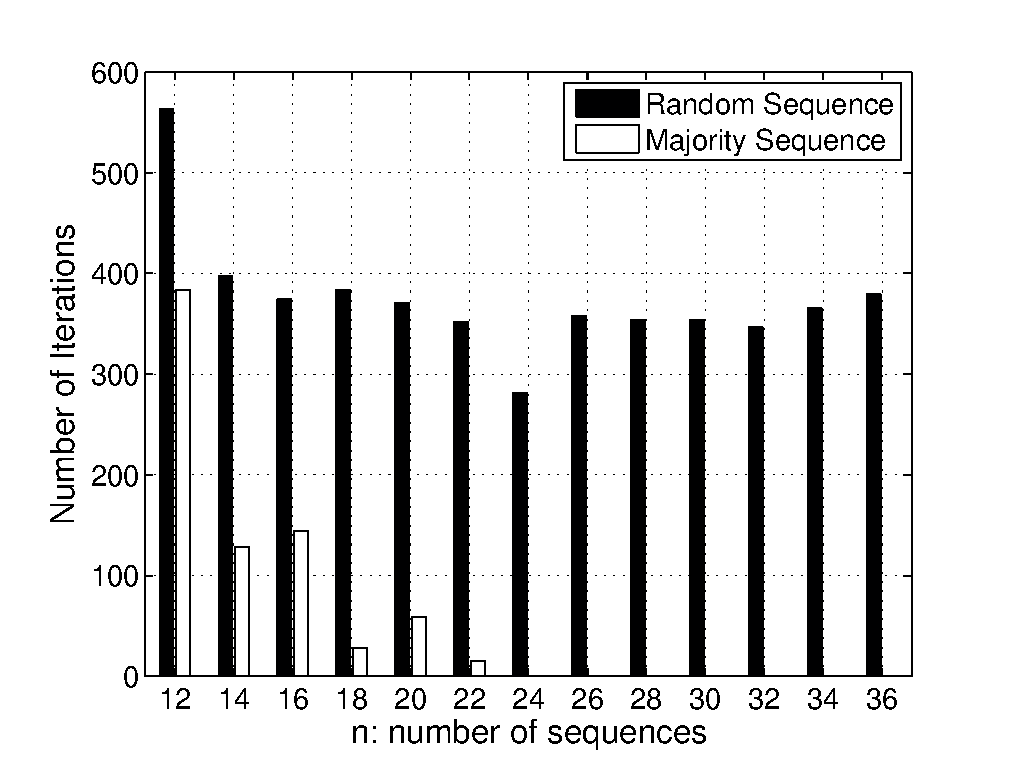
\includegraphics[width=\linewidth]{images/maj_vs_rand}% picture filename
 \caption[A comparison between the number of augmentations required to obtain a center string when procedure {\em augment} begins with a random string, and that required when procedure {\em augment} begins with a majority string, for various values of $n$.]{A comparison between the number of augmentations required to obtain a center string when procedure {\em augment} begins with a random string (shown in black), and that required when procedure {\em augment} begins with a majority string (shown in white), for various values of $n$. In all experiments, we have $\ell$ and $d$ equal to 15 and 4, respectively.}
\label{maj_vs_rand_fig}
\end{figure}

Figure \ref{maj_vs_rand_fig} demonstrates that the number of augmentations required to obtain a center string is significantly larger if $s_{maj, 0}$ is initialized to be a random string, rather than a majority string. Further, as the value of $n$ increases the disparity between the number of required number of augmentations of a majority string to obtain a center string and the required number of augmentations of a random string to obtain a center string increases substantially.  In particular, when $n$ is equal to 24 the number of augmentations required of the majority string is equal to 0 (as seen in Figure \ref{maj_vs_rand_fig}) -- illustrating that the majority string is a center string for all motif sets considered.  We observe that this fact cannot be extended to be true for random strings.
 
\begin{figure}[h!]
\centering
\includegraphics[width=\linewidth]{images/graph2v2}% picture filename
 \caption[An illustration of the decrease in the mean distance between a majority and center string as $n$ increase, for various values of $\ell$ and $d$.]{An illustration of the decrease in the mean distance between a majority and center string as $n$ increase, for various values of $\ell$ and $d$. Each line represents the mean Hamming distance for differing values of $n$. }
\label{fig2}
\end{figure}
 
Next, we considered the change in the Hamming distance as the values $n$, $\ell$, and $d$ varied.  We considered three different value of $\ell$ and $d$, varied the value of $n$ from 5 to 25, generated 100 random motif instances, and determined the mean Hamming distance between a majority string and a center string.  Figure \ref{fig2} illustrates this data and demonstrates a drastic decrease in the Hamming distance between the majority string and the center string as $n$ increases, for all the $(\ell, d)$-motif problems considered.  When the value of $n$ is significantly large, the distance between the majority string and the center string is equal to zero -- implying the majority string is a center string. 

Hence, the experimental results in this subsection illustrate the following trend: regardless of the value of $\ell$ and $d$ considered, for significantly large values of $n$ the majority string is likely to be a center string. 

\subsection{Empirical Evaluation of CSP-Greedy} 

{\em CSP-Greedy} begins with a string chosen at random from all majority strings, $s_{maj, 0}$, and iteratively augments $s_{maj, 0}$ so each time it is closer to at least one of the strings in $S$.  We consider how the number of augmentations of $s_{maj, 0}$ required to obtain a center string is affected if $s_{maj, 0}$ is initialized to a majority string, rather than a random string. 


 
\begin{table*}[h!]
\begin{center} {
	\begin{tabular}{|c|c|c||c|c|c| }
     \hline	
	$n$				& Mean accuracy 			& Mean number of		 & $n$ 			& Mean accuracy			&	Mean number of  \\
						&  						& augmentations	 & 	 			& 							& augmentations \\
	\hline
    4						& 57 			& 416 	& 16				&	99 				&	256			\\
	6  					& 86 			& 540 	& 18				&	100 				& 0\\
	8		 				& 87 			& 832 	& 20				& 100 							& 0 \\
	10					& 92 			& 800 	& 22				& 	100								& 0 \\
	12					& 98 			& 288 	& 24				& 	100 								& 0 \\
	14					& 98 			& 392 	& 26				& 	100 								& 0 \\
	\hline
	\end{tabular}}
\end{center}
\caption[Data illustrating the change in the accuracy and efficiency of {\em CSP-Greedy} as the value of $n$ increases.]{Data illustrating the change in the accuracy and efficiency of {\em CSP-Greedy}  as the value of $n$ increases.  We varied the value of $n$, and fixed $\ell$ and $d$ to be 10 and 3, respectively. We generated 1000 motif sets for each value of $n$, determined the number of augmentations of procedure {\em augment} to obtain a center string from a majority string, and calculated the mean of these 1000 values.}
\label{table2}
\end{table*} 

\subsubsection{Number of Input Strings}

The number of strings has a substantial effect on the running time of {\em CSP-Greedy}. Table \ref{table2} outlines the relationship between the value of $n$ and the accuracy and efficiency of {\em CSP-Greedy}. The mean accuracy of the algorithm is the percentage of motif sets where {\em CSP-Greedy} finds a center string.  We varied the value of $n$, and fixed $\ell$ and $d$ to be 10 and 3, respectively. We generated 1000 motif sets for each value of $n$, determined the number of augmentations of procedure {\em augment} to obtain a center string from a majority string, and calculated the mean of these 1000 values.  For this set of experiments we increased the maximum of augmentations to 1000.  Table \ref{table2} shows that when $n$ becomes significantly large ({\em i.e.}\ $n$ is equal to 18) the majority string is a center string.  
 
 
Figure \ref{fig:csp_greedy_plot_v2} illustrates the change in the running time of algorithm as $n$ increases.  Even for significantly large value of $\ell$ and $d$ ({\em i.e.}\ when $\ell$ was equal to 29 and $d$ was equal to 10), the algorithm ran extremely efficiently.  For each set of values of $n$, $\ell$, and $d$, 1000 motif sets were generated, {\em CSP-Greedy} was ran on each set, and the mean running time was recorded.  The running time decreases significantly as $n$ increased for all values of $\ell$ and $d$ considered.  Out of all the motif sets we considered, a center string was not obtained for 21 of these sets.   

\begin{figure}[h!]
\centering
\includegraphics[width=65mm,trim=7cm 8cm 7cm 7cm]{images/csp_greedy_running_v2}% picture filename
 \caption[An illustration of the time required by {\em CSP-Greedy} to obtain a center string as $n$ increases, for various values of $\ell$ and $d$.]{An illustration of the time required by {\em CSP-Greedy} to obtain a center string as $n$ increases, for various values of $\ell$ and $d$.}
\label{fig:csp_greedy_plot_v2}
\end{figure}

\subsubsection{Length/Degeneracy Ratio}

We consider the change in the accuracy as $\ell$ and $d$ increase.  Again, we generated 1000 random motif sets, and obtained the mean accuracy and number of augmentations from running Procedure {\em augment} (with the number of augmentations increased to 1000).  Table \ref{closest_string_chapter:table1} illustrates the data from these experiments and shows that when $n = 20$ the mean number of augmentations was equal to zero for majority of values of $\ell$ and $d$, implying that the majority string was a center string.

\begin{table*}[h!]
\begin{center}{ 
\begin{tabular}{|cc||c|c|}
\hline
 		&  			& \multicolumn{2}{c|}{$n = 5$} \\
\hline
$\ell$ 		& $d$ 		& Mean accuracy 		& Mean number of augmentations\\
\hline
\hline
   6			& 1			& 97 			& 270 			 \\
	8  		& 2			& 83 			& 272	 		\\
	10		& 3 			& 67 			& 825 			\\
	12		& 3			& 86 			& 504 			\\	
	14		& 4			& 63 			& 813 		 \\
	15		& 4			& 69 			& 744 		 \\
	18		&	6			& 61 			& 920 		 \\
	21		& 7			& 62 			& 912 		 \\
\hline
		&			& \multicolumn{2}{c|}{$n = 15$}  \\
\hline
   6			& 1			& 100 			& 0				 \\
	8  		& 2			& 100 			& 0 				 \\
	10		& 3 			& 99			& 225	 				\\
	12		& 3			& 100 			& 0 				 \\	
	14		& 4			& 99 			& 440	 		\\
	15		& 4			& 99  			& 506	 \\
	18		&	6			& 96 			& 916	 \\			
	21		& 7			& 93 			& 945	 \\
\hline
&& \multicolumn{2}{c|}{$n = 20$} \\
\hline
   6			& 1				& 100  		& 0 \\
	8  		& 2				& 100  		& 0 \\
	10		& 3 			& 100  		& 0	\\
	12		& 3				& 100  		& 0 \\	
	14		& 4		& 100  		& 0 \\
	15		& 4			& 100  		& 0 \\
	18		&	6							& 96 		& 183 \\
	21		& 7				& 97  		& 291 \\
\hline
\end{tabular} }
\end{center}
\caption[Data illustrating the change in the accuracy and efficiency of {\em CSP-Greedy} as $\ell$ and $d$ increase.]{Data illustrating the change in the accuracy and efficiency of {\em CSP-Greedy} as $\ell$ and $d$ increase.The mean accuracy and number of augmentations represents the results obtained for 1000 randomly generated motif sets.}
\label{closest_string_chapter:table1}
\end{table*} 
\newpage

Figure \ref{fig:csp_greedy_plot} illustrates the change in the running time of {\em CSP-Greedy} as $\ell$ and $d$ vary, and $n$ is fixed at 20.  When the $\ell / d$ ratio became significantly large the running time was infinitesimal.  Again, for each set of values of $n$, $\ell$, and $d$, 1000 motif sets were generated, {\em CSP-Greedy} was run on each set, and the mean running time was recorded.  Out of the 24,000 sets considered, a center string was not obtained for 42 of the sets.   

\begin{figure}[h!]
\centering
\includegraphics[width=65mm,trim=7cm 8cm 7cm 7cm]{images/csp_greedy_running_time_v1}% picture filename
 \caption[An illustration of the time required by {\em CSP-Greedy} to obtain a center string as $\ell/d$ ratio increases, for various values of $d$.]{An illustration of the time required by {\em CSP-Greedy} to obtain a center string as $\ell/d$ ratio increases, for various values of $d$. In these experiments, $n$ is equal to 20. }
\label{fig:csp_greedy_plot}
\end{figure}


\subsection{Application to Motif Recognition} 

MCL-WMR was developed specifically for the problem of detecting weak motifs in genetic data and works by first building a weighted graph model of the given motif-recognition problem and then using a graph clustering algorithm to quickly determine important subgraphs that need to be searched further for valid motifs. These smaller subproblems are then solved optimality using a dynamic-programming algorithm for finding motifs in dense subgraphs.  We extend MCL-WMR to incorporate {\em CSP-Greedy}. This new algorithm, {\em pMCL-WMR}, detects motifs in data sets with a large number of strings.  More specifically, pMCL-WMR efficiently discovers motifs in data sets that have 30 or more strings, and finds regulatory strings in genomic data.  

\subsection{Performance of pMCL-WMR on Synthetic Data}

We produced problem instances as follows: we chose a random center string of length $\ell$, and picked $m$ occurrences of the motif by randomly choosing $d$ positions per occurrence and randomly mutating the base at each. We constructed $m$ background strings of length $n$ and inserted the generated motifs into a random position in the string.  For each of the $(\ell, d)$ combinations, 100 random sets of input strings ($n = 20$, $m = 1000$) were generated. The running time is given in CPU seconds.  

Table \ref{table3} shows the comparison between the running time of MCL-WMR and that of pMCL-WMR. Two significant trends are witnessed in the data: pMCL-WMR is capable of solving hard instances of motif recognition ({\em i.e.}\ when $\ell = 25$ and $d = 7$) and pMCL-WMR gives a dramatic improvement over MCL-WMR with respect to the running time for all values of $\ell$ and $d$. The main advantage to our tool is the time required to solve the extremely difficult challenge problems -- from the $(18, 6)$ to the $(25, 7)$ problem -- in substantially better running time and with 100\% accuracy. 

The computational results in Subsection \ref{sec:cspgreedy_vs_fpt} inspire the investigation of instances with a significantly large number of sequences -- that is, instances where $n$ varies from values greater than 20. Table \ref{table4} shows the evaluation of the performance of pMCL-WMR on a range of problems with an increasing number of sequences.  The efficiency on these sets of problems is noteworthy ranging from 781 (when $n = 18$) to 2781 ($n = 30$). As far as we are aware, these are the first computational experiments where $n$ is larger than 20. 

An entry ``-'' indicates that the program was unable to solve the specific problem in a reasonable amount of time. The mean running time is given, followed by the standard deviation. 

\begin{table*}[h]
\begin{center} {
	\begin{tabular}{|c|c|c|}
     \hline	
	$(\ell, d)$	 		& MCL-WMR		& pMCL-WMR	 \\
	\hline
    (10, 2)				& 1003 / 32 		& 518 / 11			\\
    (15, 4)				& 3232 / 92			& 788 / 22			\\
	(16, 5)  			& 4200 / 103		& 1529 / 31				\\
	(18, 6)		 		& 8905 / 150		& 1723 / 47 			\\
	(25, 7)				& -						& 	2923 / 45		\\
	\hline
	\end{tabular}} 
	\end{center}
\caption[Comparison between the performance of MCL-WMR and that of pMCL-WMR on synthetic data. ]{Comparison between the performance of MCL-WMR and that of pMCL-WMR on synthetic data. In all experiments, $m = 1000$, $n = 20$, and $\ell$ and $d$ are varied. The mean and standard deviation of the running time in CPU seconds is given. }
\label{table3}
\end{table*}


\begin{table*}[h]
\begin{center} {
  \begin{tabular}{|c|c|c|c|}
     \hline	
	$n$				& MCL-WMR 	& pMCL-WMR	 \\
	\hline
    18				& 1981 / 65		& 781 / 23 \\
	20  				& 3233 / 82  	& 931 / 45 \\
	24		  	  	&	-					& 1721	/ 72	\\
	28				&  - 					& 1200	/ 87 \\
	30				&  - 					& 2781	/ 91		 \\
	\hline
	\end{tabular}}
\end{center}
	\caption[Comparison between the performance of MCL-WMR and that of pMCL-WMR on synthetic data as $n$ increases.]{Comparison between the performance of MCL-WMR and that of pMCL-WMR on synthetic data as $n$ increases. In all experiments, $\ell = 15$, $d = 4$ and $m = 1000$. The mean and standard deviation of the running time in CPU seconds is given. } 
	\label{table4}
\end{table*}
 	
\subsection{Using pMCL-WMR to Find Regulatory Elements}

An important biological challenge is to determine regulatory elements in DNA -- specifically, binding sites for transcription factors.  In this section, we demonstrate the use of pMCL-WMR in discovering these DNA sequence ``motifs'' in data sets with a large number of DNA sequences. Tompa {\em et al.}\ \cite{tompa} extensively assess 13 motif-recognition tools using test sets that make use of transcription factor binding sites. The binding sites were obtained from the TRANSFAC database \cite{WDKK96} and contain eukaryotic transcription factors.  The TRANSFAC database is extremely comprehensive, containing data from a large variety of species ({\em i.e.}\ species include yeast, {\em mus}, {\em oryctolagus cuniculus}, and {\em homo sapiens}) \cite{WDKK96}. For more details concerning the data set, including the selection process for transcription factors and binding sites from TRANSFAC, see Tompa {\em et al.}\ \cite{tompa}.  

Each transcription factor gives rise to one set of sequences. The number of sequences varied from 34 to 6 and the sequence length (parameter $m$) varied from 700bp to 2000bp. The transcription factor binding sites vary in length and thus, in order to assess pMCL-WMR, we ran the program on varied values $\ell$ and $d$.  The lengths of the motifs were same as those of the published motifs and $d$ varied.  Experimental results are shown in Table \ref{bio_table}.  pMCL-WMR was capable of discovered all of the motifs sets reported by Tompa {\em et. al.}\ \cite{tompa}, as well as some undetected motifs.  The motifs discovered only by pMCL-WMR and not by  any of the motif-recognition programs assessed by Tompa {\em et. al.}\ \cite{tompa} are shown in Table \ref{bio_table}. 

\begin{table*}[h]
\begin{center} {
	\begin{tabular}{|c|c|c|c|}
     \hline	
	Data set 	& $(\ell, d)$ & $n$ & Motif pattern discovered  \\
	\hline
	hm06		& (7, 1) &	9	 & TttTccC		   \\
	hm06		& (8, 1) & 9 & GGAcTGCT		    \\
	hm10		& (8, 3) & 6 & TTTcgCGC		  \\	
	hm13		& (10, 2) & 6 & aaAATTatTC		   \\
	hm13		& (11, 1) & 6	 & tccCcCACAaa		    \\
	hm19		& (11, 2) & 5 & tccCcCACAaa		    \\ % check this
	\hline			
   	\end{tabular}}
\end{center}
\caption[Illustration of the regulatory strings found by pMCL-WMR]{Illustration of the regulatory strings found by pMCL-WMR. Data are collected from SCPD.  For each set of data, we determined motifs of the same length using pMCL-WMR, and gave the motif published by Tompa {\em et. al.} \cite{tompa} for the same data set.  }
\label{bio_table}
\end{table*}


\begin{table*}[h]
\begin{center} {
	\begin{tabular}{|c|c|c|c|}
     \hline	
	Data set	& $(\ell, d)$ & $n$& Time \\
	\hline
	hm06		& (7, 1) &	9		& 80 \\
	hm06		& (8, 1) & 9		& 102 \\
	hm10		& (8, 3) & 6		& 210\\	
	hm13		& (10, 2) & 6		& 178 \\
	hm13		& (11, 1) & 6		& 220 \\
	hm19		& (11, 2) & 5		& 321\\ % check this
	\hline			
   	\end{tabular}}
\end{center}
\caption[CPU time required by pMCL-WMR to detect the regulatory sequence patterns shown in Table \ref{bio_table}]{CPU time required by pMCL-WMR to detect the regulatory sequence patterns shown in Table \ref{bio_table}.}
\label{bio_table:runtime}
\end{table*}

\section{Summary and Open Problems}

In this chapter, we gave a linear-time algorithm for solving {\sc Closest String} problem with four binary strings, proved lower and upper bounds for the approximation guarantees for a simple probabilistic algorithm for the general problem, and showed the existence of an algorithm with running time $O(\ell^3)$ that achieves a $\left(1  - \left( \frac{\epsilon}{ 2^{n}} \right)^{\ell}\right)$-approximation, for some small $\epsilon > 0$ and significantly large values of $n$.  Our smoothed analysis of {\em CSP-Greedy} gives reasons as to why this algorithm and the $O(n\ell + nd \cdot d^d)$-time algorithm of Gramm {\em et al.}\ \cite{GNR03} is efficient in practice for {\sc Closest String} instances with a large number of strings. This analysis gives an analytical reason to why this -- and perhaps other similar {\sc Closest String} algorithms -- perform well in practice.  Lastly, we gave empirical results that demonstrate the majority string is likely to be a center string when the number of sequences is moderately large.  

There exist numerous open problems that warrant further investigation, including the following:

\begin{itemize}
\item Since the publication of the linear-time algorithm presented in this chapter, these results have been extended by Amir {\em et al.}\ \cite{amir} to a variant of the {\sc Closest String} problem. Determining how these results could be generalized to larger alphabets or to instances containing more than four strings remains open. Such a generalization would invite many open problems in motif recognition to be revisited, as their tractability might be determined more concretely. 

\item In smoothed analysis one often analyzes how fragile worst case instances are. Manthey and Reischuk \cite{MR05} suggest examining the dual property of how robust the best (or good) instances are.  Lastly, we propose continuing this form of analysis and determining how stable the best-case instances of the closest string problem are under perturbations. This would involve considering instances where {\em CSP-Greedy} performs efficiently and showing that even large perturbations of these instances yield problems that can be solved in efficient time.

\item There exist several open problems related to the smoothed complexity of string selection problems that warrant investigation.  Analyzing the smoothed complexity of the PTAS of Li {\em et al.}\ \cite{LMW02} for the {\sc Closest String} problem requires further study.  The running time of this PTAS is detrimentally large, thus reducing the algorithm to only theoretical importance.  However, there have been several papers attempting to prove that the algorithm performs significantly better in practice \cite{brona1,brona2}; the smoothed analysis of the algorithm would potentially complete this area of study.
\end{itemize}